\documentclass[11pt]{article}
\usepackage[margin=1in]{geometry}
\usepackage{amsmath,amssymb}
\usepackage{graphicx}
\usepackage{booktabs}
\usepackage{longtable}
\usepackage{xcolor}
\usepackage{tikz}
\usetikzlibrary{arrows.meta,positioning,shapes.geometric,fit,calc,decorations.pathmorphing}
\usepackage{listings}
\usepackage{hyperref}
\usepackage{caption}
\usepackage{subcaption}

\lstset{basicstyle=\ttfamily\small, columns=fullflexible, frame=single,
        backgroundcolor=\color{gray!6}, keywordstyle=\color{blue!60!black}\bfseries,
        commentstyle=\color{green!40!black}, showstringspaces=false, breaklines=true}

\setlength{\emergencystretch}{3em}
\newcommand{\Scap}{S_{\mathrm{cap}}}
\newcommand{\Qsafe}{Q_{\mathrm{safe}}}
\newcommand{\code}[1]{\texttt{#1}}

\title{Learning Reservoir Operating Rules with Reinforcement Learning:\\
       a Tutorial with OpenHydroQual as the Simulator}
\author{OpenHydroQual-RL working notes}
\date{\today}

\begin{document}
\maketitle

\begin{abstract}
This report teaches reinforcement learning (RL) through a worked water
resources example. RL is a way of \emph{learning an operating rule by
trial and error in a simulator}. Here the simulator is an OpenHydroQual
(OHQ) model, driven from Python, and the learner is a small neural network
trained with PyTorch. We start with a single water-supply reservoir hit by
random storms. Each day the learned rule chooses a release that must
balance meeting a downstream demand against flooding the river and
spilling water. We then move to a harder problem: two reservoirs in series
with an uncontrolled tributary. Along the way we explain the RL concepts
from the ground up, relating them to stochastic dynamic programming and
model calibration. We also document the engineering: how the OHQ model is
built from Python, how its output was verified against an exact solution
(which uncovered and led to fixing two issues in OHQ), how training is
parallelized, and how the learned rules compare with classical rule
curves. No prior knowledge of RL is assumed; familiarity with hydrologic
modeling and basic calculus and probability is.
\end{abstract}

\paragraph{How to read this report.} Section~\ref{sec:primer} is a
self-contained introduction to RL. Its first half is conceptual, and its
last part (Section~\ref{sec:primer_math}) gives the mathematics. Sections 3
to 5 set up the first problem and the simulator. Section~\ref{sec:ppo}
explains the learning algorithm (PPO) step by step. Section~\ref{sec:results}
shows the results. Section~\ref{sec:cascade} repeats everything for the
harder two-reservoir problem. A nomenclature list is at the front and an RL
glossary at the end.

\tableofcontents
\newpage

\section*{Nomenclature}
\addcontentsline{toc}{section}{Nomenclature}
Units: volumes in m$^3$, flows in m$^3$/d, time in days. Because each
decision step is one day, a volume over a step (m$^3$) and the mean flow
over that step (m$^3$/d) are numerically equal; this is why volumes are
compared directly with $\Qsafe$ and $D_t$.

\begin{longtable}{@{}p{0.19\textwidth}p{0.58\textwidth}p{0.15\textwidth}@{}}
\toprule
Symbol & Meaning & Value / unit\\
\midrule
\endhead
\multicolumn{3}{@{}l}{\emph{Time and indices}}\\
$t$ & time; as a subscript, the day index of a decision step covering $[t,t+1]$ & d\\
$T$ & episode (season) length & 90 steps\\
$t_0$ & start time of one OHQ simulation interval & d\\
$k$ & forecast lead time & 1, 2, 3 d\\
$j$ & storm index & --\\
$\tau$ & time since the onset of a storm, $t-t_j$ & d\\
$\Delta t_0$ & OHQ initial (and, in the environment, fixed) time step, \code{initial\_time\_step} & 0.05 d\\
$\Delta t$ & decision interval (one day) & 1 d\\[3pt]
\multicolumn{3}{@{}l}{\emph{Reservoir and structures}}\\
$S(t),\,S_t$ & reservoir storage (continuous; at the start of day $t$) & m$^3$\\
$S_0$ & initial storage of an episode, $\sim U(0.3,0.8)\Scap$; also of a single simulation interval & m$^3$\\
$\Scap$ & storage at the spillway crest (capacity) & 50{,}000 m$^3$\\
$S_{dead}$ & storage below which the outlet release tapers to zero & 200 m$^3$\\
$Q_t$ & release requested by the policy for day $t$ & m$^3$/d\\
$Q_{\mathrm{out}}$ & outlet capacity (maximum release) & 6{,}000 m$^3$/d\\
$\Qsafe$ & safe capacity of the downstream channel & 3{,}000 m$^3$/d\\
$Q_{\min},Q_{\max},$\newline$S_{\min},S_{\max}$ & parameters of the OHQ \code{Reservoir\_link\_rule} flow rule (Section~\ref{sec:ohqmodel}) & --\\
$Q(S)$ & flow of a \code{Reservoir\_link\_rule} link as a function of storage & m$^3$/d\\
$V^{in}_t,V^{rel}_t,V^{sp}_t$ & inflow, released and spilled volume during day $t$ & m$^3$\\[3pt]
\multicolumn{3}{@{}l}{\emph{Forcing}}\\
$Q_{in}(t)$ & reservoir inflow & m$^3$/d\\
$q_b$ & mean base flow & 600 m$^3$/d\\
$\beta$ & per-episode base-flow factor, $\sim U(0.7,1.3)$ & --\\
$h_j(t)$ & hydrograph of storm $j$ & m$^3$/d\\
$t_j$ & onset time of storm $j$ (probability 0.06 per day) & d\\
$P_j$ & peak flow of storm $j$, $\sim U(5000,15000)$ & m$^3$/d\\
$t_r$ & storm rise time & 0.5 d\\
$k_j$ & recession constant of storm $j$, $\sim U(0.3,0.7)$ & d$^{-1}$\\
$D(t),\,D_t$ & downstream demand (on day $t$) & m$^3$/d\\
$\bar D$ & mean demand & 1{,}500 m$^3$/d\\
$\psi$ & demand phase, $\sim U(0,2\pi)$ & rad\\
$\hat F_{t+k}$ & forecast, issued on day $t$, of the daily-mean inflow on day $t+k$ & m$^3$/d\\
$\sigma_F$ & log-normal forecast error scale, $0.2\sqrt{k}$ & --\\
$\xi$ & all random elements of a season (storms, $\beta$, $\psi$, forecast errors, $S_0$) & --\\[3pt]
\multicolumn{3}{@{}l}{\emph{MDP, reward and objective}}\\
$o_t$ & observation (7 normalized features, Section~\ref{sec:mdp}) & --\\
$a_t$ & action in $[-1,1]$; $Q_t=\tfrac12(a_t+1)Q_{\mathrm{out}}$ & --\\
$r_t$ & reward of day $t$ & --\\
$r_T^{\mathrm{term}}$ & terminal (end-of-season storage) reward & --\\
$w_f,\,w_s,\,w_T$ & weights of the flood, spill and terminal penalties & 2, 1, 5\\
$J(\pi)$ & objective: expected undiscounted season return, Eq.~\eqref{eq:objective} & --\\
$J_\gamma(\pi)$ & discounted return maximized during training & --\\
$\eta$ & flood-rule threshold of the rule-curve baselines (fraction of $\Scap$) & 0.8; tuned 0.4\\[3pt]
\multicolumn{3}{@{}l}{\emph{PPO}}\\
$\pi_\theta(a\mid o)$ & stochastic (Gaussian) policy with network parameters $\theta$ & --\\
$\mu_\theta(o)$ & mean of the policy (actor network output) & --\\
$\sigma$ & standard deviation of the policy (learned, state-independent) & $0.59\to0.15$\\
$V_\phi(o)$ & value function (critic network) with parameters $\phi$ & --\\
$\gamma$ & discount factor & 0.99\\
$\lambda$ & GAE parameter & 0.95\\
$\delta_t$ & temporal-difference error & --\\
$\hat A_t$ & advantage estimate (GAE), normalized per update & --\\
$\hat R_t$ & return target for the critic, $\hat A_t+V_\phi(o_t)$ & --\\
$d_t$ & episode-end flag (1 on the last step of a season) & 0/1\\
$\rho_t$ & probability ratio of the new to the old policy & --\\
$\epsilon$ & PPO clipping parameter & 0.2\\
$c_v$ & value-loss coefficient & 0.5\\
$L(\theta)$ & PPO loss minimized by gradient descent & --\\[3pt]
\multicolumn{3}{@{}l}{\emph{Two-reservoir cascade (Section~\ref{sec:cascade})}}\\
$S^A_t,\,S^B_t$ & storage of reservoir A (upstream) and B (downstream) & m$^3$\\
$S^A_{cap},\,S^B_{cap}$ & capacities (spillway crests) of A and B & 60{,}000; 30{,}000 m$^3$\\
$S^A_n$ & storage of A at the end of solver step $n$ within a day & m$^3$\\
$Q^A_t,\,Q^B_t$ & releases requested by the policy for A and B & m$^3$/d\\
$Q^A_{\mathrm{out}},\,Q^B_{\mathrm{out}}$ & outlet capacities of A and B & 6{,}000; 8{,}000 m$^3$/d\\
$Q^A_{in},Q^B_{in},Q^{tr}$ & inflow to A, to B, and tributary flow & m$^3$/d\\
$q^B_t,\,q^{tr}_t$ & current (start-of-day) inflow to B and tributary flow & m$^3$/d\\
$\bar P_c$ & storm peak scale of catchment $c$ & m$^3$/d\\
$m$ & intensity of a regional storm, common to all catchments, $\sim U(0.5,1.5)$ & --\\
$V^{rel,A}_t,V^{sp,A}_t$ & released and spilled volume of A during day $t$ (enter B) & m$^3$\\
$V^{rel,B}_t,V^{sp,B}_t$ & released and spilled volume of B during day $t$ & m$^3$\\
$V^{tr}_t$ & tributary volume during day $t$ & m$^3$\\
$V^{riv}_t$ & river volume at the flood point, $V^{rel,B}_t+V^{sp,B}_t+V^{tr}_t$ & m$^3$\\
$Q^{sup}_t$ & part of the demand the tributary does not supply (rule) & m$^3$/d\\
$\eta_A,\,\eta_B$ & thresholds of the cascade rule (fractions of $S^A_{cap}$, $S^B_{cap}$) & --\\[3pt]
\multicolumn{3}{@{}l}{\emph{Stormwater pond (Section~\ref{sec:pond})}}\\
$h$ & pond depth & m\\
$\alpha,\beta$ & pond storage--depth parameters, $S\approx\alpha h^\beta$ & 250; 2\\
$u_t$ & valve opening chosen by the policy for hour $t$ & 0--1\\
$C_d,\,A_{max}$ & valve discharge coefficient; orifice area at full opening & 0.6; 0.03 m$^2$\\
$\varepsilon$ & regularization head of the valve law & 1 mm\\
$Q(t),\,Q_n$ & pond outflow (valve + overflow); at solver step $n$ & m$^3$/d\\
$\delta t$ & OHQ solver step (5 minutes) & d\\
$Q_p$ & outflow exceeded a fraction $p$ of the time & m$^3$/d\\
$p$ & exceedance probability & 0.001\\
$\lambda$ & decay rate of the Laplace age tracer & 1 d$^{-1}$\\
$\tau,\,p(\tau)$ & water age and its probability density & d\\
$C$ & age-tracer concentration, $\mathcal L\{p\}(\lambda)=E[e^{-\lambda\tau}]$ & --\\
$F_y$ & young-water fraction of the outflow (flow-weighted $C$) & --\\
$J$ & pond evaluation objective, $Q_p/Q_p^{\,passive}+F_y/F_y^{\,passive}$ (lower is better; passive pond = 2) & --\\
$Q_p^{\,passive},F_y^{\,passive}$ & $Q_p$ and $F_y$ of the passive pond (valve fully open) under the same rain & --\\
$a_t$ (pond) & network action; valve opening $u_t=((a_t+1)/2)^2$ & --\\
$Q_{ref},\,V_{ref}$ & reference flow and volume of the pond reward & 1{,}000 m$^3$/d; 1{,}000 m$^3$\\
$w_q,\,w_y$ & weights of the peak-flow surrogate and the young-water terms & 1; 5\\
$u_{hold},u_{pre}$ & openings of the forecast rule (holding; pre-release) & --\\[3pt]
\multicolumn{3}{@{}l}{\emph{Other}}\\
$U(a,b)$ & uniform distribution on $[a,b]$ & --\\
$\mathcal N(\mu,\sigma^2)$ & normal distribution & --\\
$\mathbb E$ & expectation & --\\
\bottomrule
\end{longtable}
\newpage

%=====================================================================
\section{Overview}
%=====================================================================

Figure~\ref{fig:architecture} shows the software stack. The RL agent
(PyTorch) talks to a Gymnasium environment through the standard
\code{reset}/\code{step} API. The environment generates the hydrologic
forcing, computes the reward and delegates the physics to a
\emph{simulator backend}. The only backend implemented so far,
\code{OHQBackend}, rebuilds and solves an OHQ model for each one-day
control interval through \code{openhydroqual\_py}, a pybind11 module that
links \code{libOHQLib}. The backend interface is deliberately narrow so
that a codegen-compiled OHQ kernel can later replace it
(Section~\ref{sec:performance}).

\begin{figure}[h]
\centering
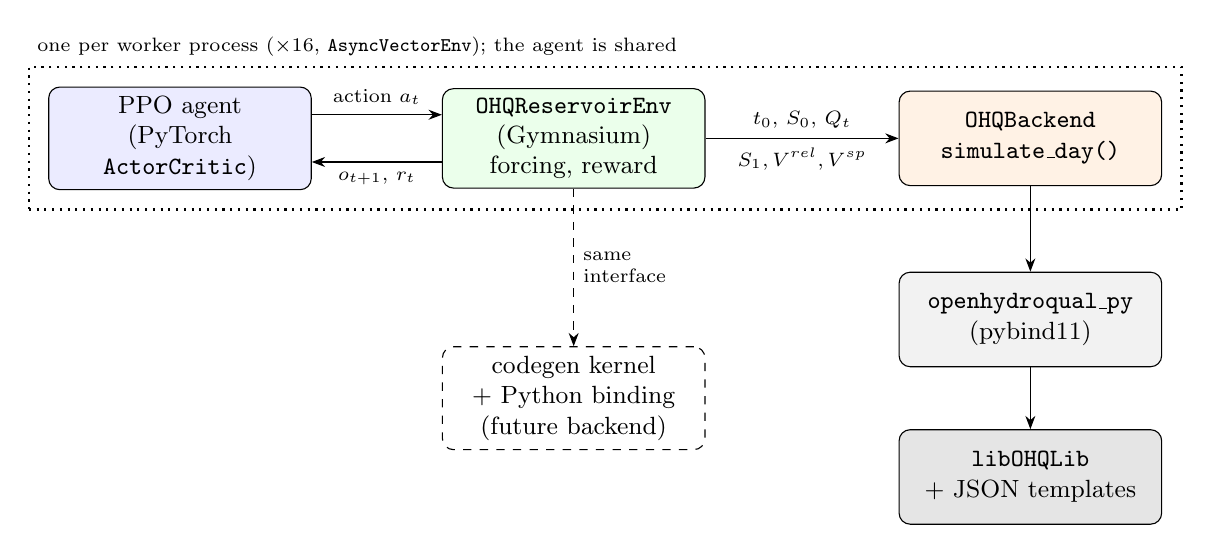
\begin{tikzpicture}[>=Stealth, font=\small,
  box/.style={draw, rounded corners, align=center, minimum height=1.2cm, text width=3.1cm, fill=#1},
  box/.default=white]
  \node[box=blue!8]   (agent) at (0,0)     {PPO agent\\(PyTorch \code{ActorCritic})};
  \node[box=green!8]  (env)   at (5,0)     {\code{OHQReservoirEnv}\\(Gymnasium)\\forcing, reward};
  \node[box=orange!10](be)    at (10.8,0)    {\code{OHQBackend}\\\code{simulate\_day()}};
  \node[box=gray!10]  (py)    at (10.8,-2.3) {\code{openhydroqual\_py}\\(pybind11)};
  \node[box=gray!20]  (lib)   at (10.8,-4.3) {\code{libOHQLib}\\+ JSON templates};
  \node[box=white, dashed] (cg) at (5,-3.3) {codegen kernel\\+ Python binding\\(future backend)};
  \draw[->] ([yshift=3mm]agent.east) -- node[above, font=\scriptsize]{action $a_t$} ([yshift=3mm]env.west);
  \draw[<-] ([yshift=-3mm]agent.east) -- node[below, font=\scriptsize]{$o_{t+1},\,r_t$} ([yshift=-3mm]env.west);
  \draw[->] (env) -- node[above, font=\scriptsize]{$t_0,\,S_0,\,Q_t$} node[below, font=\scriptsize]{$S_1,V^{rel},V^{sp}$} (be);
  \draw[->] (be) -- (py);
  \draw[->] (py) -- (lib);
  \draw[->, dashed] (env) -- node[right, font=\scriptsize, align=left]{same\\interface} (cg);
  \node[draw, dotted, thick, fit=(agent)(env)(be), inner sep=7pt] (w) {};
  \node[anchor=south west, font=\scriptsize] at (w.north west) {one per worker process ($\times16$, \code{AsyncVectorEnv}); the agent is shared};
\end{tikzpicture}
\caption{Software architecture. Each vectorized worker process owns one
environment, one backend and its own OHQ working folder.}
\label{fig:architecture}
\end{figure}

\paragraph{Files.}
\begin{itemize}\itemsep0pt
  \item \code{ohq\_reservoir\_env.py} -- \code{OHQBackend}, \code{OHQReservoirEnv}, rule-curve baseline.
  \item \code{train\_ppo.py} -- PPO with GAE in plain PyTorch, parallel rollouts.
  \item \code{evaluate.py} -- comparison against baselines, figures and table.
  \item \code{diagnostics.py} -- simulator verification and timing figures.
  \item \code{report/} -- this document.
\end{itemize}

%=====================================================================
\section{Reinforcement learning in a nutshell}\label{sec:primer}
%=====================================================================

This section explains the ideas behind reinforcement learning (RL) for a
reader who knows hydrologic modeling and calibration but has not used RL.
Everything later in the report builds on it. The glossary at the end of the
report collects the terms.

\subsection{What problem does RL solve?}
Think of a reservoir operator. Every morning they look at the reservoir
level, the current inflow and the weather forecast, and decide how much
water to release today. Tomorrow they see the consequences and decide
again. The goal is not to make each single day look good. It is to do well
over the whole season: to meet demand, avoid floods and not waste water
over the spillway. The operator does not know the future storms, so a good
decision now must hedge against many possible futures.

This is a \emph{sequential decision problem under uncertainty}. RL is a
family of methods that \emph{learn a decision rule for such problems by
trial and error}: they try decisions in a simulator, observe what happens
and gradually improve the rule. In this report, the simulator is an
OpenHydroQual model.

\paragraph{How this differs from calibration.} In model calibration we
search for \emph{parameter values} that make a model fit observed data
(for example with a genetic algorithm or Levenberg--Marquardt). In RL we
search for a \emph{decision rule}, called a \emph{policy}: a function that
maps what the operator sees to what the operator does. The rule is judged
by how well it performs over many simulated futures, not by how well it
fits data.

\paragraph{Why not just optimize the release schedule?} One could fix a
storm sequence and optimize the 90 daily releases for it. But real storms
are unknown in advance. A schedule that is optimal for one storm sequence
can be disastrous for another: it might release water ahead of a storm that
never comes. What we need is a rule that \emph{reacts} to what it observes
(closed-loop control) instead of a fixed plan (open-loop control). Classical
alternatives each have a catch:
\begin{itemize}\itemsep1pt
\item \textbf{Rule curves} are hand-designed rules with a few parameters
(for example, ``release extra water above 80\% full''). They are simple and
transparent but limited to the shape the designer chose.
\item \textbf{Stochastic dynamic programming} finds the optimal rule
exactly, but its cost explodes with the number of state variables (the
``curse of dimensionality''). The cascade in Section~\ref{sec:cascade} has
16 observed quantities, far beyond what it can handle.
\item \textbf{Model predictive control} re-optimizes a plan every day over
a forecast horizon. It needs a fast optimizer inside the loop and a model
of forecast uncertainty.
\end{itemize}
RL instead learns a flexible rule (here a small neural network) directly
from simulations. The price is that it needs a lot of them, hundreds of
thousands of simulated days here, which is why simulator speed matters
(Section~\ref{sec:performance}).

\subsection{The agent--environment loop}
RL describes the problem as a loop between an \emph{agent} (the decision
maker) and an \emph{environment} (everything else) (Figure~\ref{fig:loop}).
At each step $t$:
\begin{enumerate}\itemsep1pt
\item the agent receives an \textbf{observation} $o_t$, the information
available for the decision (storage, inflow, forecasts, demand, \dots);
\item it chooses an \textbf{action} $a_t$ (here, today's release);
\item the environment advances one step (here, OHQ simulates one day) and
returns a \textbf{reward} $r_t$, one number that scores how good that step
was, together with the next observation $o_{t+1}$.
\end{enumerate}
A sequence of steps from a start to an end is an \textbf{episode}; here one
episode is one 90-day season with its own random storms. The sum of the
rewards over an episode is the \textbf{return}. The agent's goal is to
choose actions that make the return as large as possible \emph{on average
over all the seasons it might face}.

\begin{figure}[h]
\centering
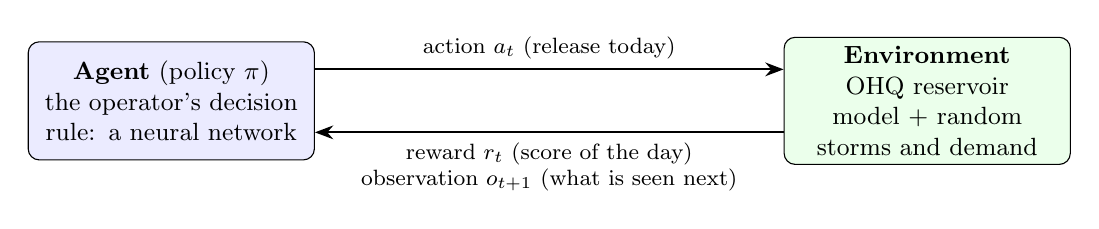
\begin{tikzpicture}[>=Stealth, font=\small,
  box/.style={draw, rounded corners, align=center, minimum height=1.5cm, text width=3.4cm, fill=#1}]
  \node[box=blue!8] (agent) at (0,0) {\textbf{Agent} (policy $\pi$)\\the operator's decision rule: a neural network};
  \node[box=green!8] (env) at (9.6,0) {\textbf{Environment}\\OHQ reservoir model + random storms and demand};
  \draw[->, thick] ([yshift=4mm]agent.east) -- node[above, align=center, font=\footnotesize]{action $a_t$ (release today)} ([yshift=4mm]env.west);
  \draw[->, thick] ([yshift=-4mm]env.west) -- node[below, align=center, font=\footnotesize]{reward $r_t$ (score of the day)\\observation $o_{t+1}$ (what is seen next)} ([yshift=-4mm]agent.east);
\end{tikzpicture}
\caption{The agent--environment loop, repeated once per simulated day.}
\label{fig:loop}
\end{figure}

\paragraph{Designing the reward is designing the objective.} The agent
optimizes exactly what the reward measures and nothing else. Here the
reward penalizes supply deficits, downstream flooding, spill and ending
the season empty (Section~\ref{sec:objective}). If a penalty were missing
the agent would ignore that concern, and if a weight were too large it
would over-react to it. Choosing the reward is the main place where
engineering judgment enters.

\paragraph{Observation versus state.} The \emph{state} is everything that
determines the future. The \emph{observation} is what the agent actually
sees. The agent never sees future storms, only noisy forecasts of them, so
it must act well despite incomplete information, exactly like a real
operator.

\paragraph{Discounting.} Many RL methods maximize a \emph{discounted}
return, $r_0+\gamma r_1+\gamma^2 r_2+\dots$, with a discount factor $\gamma$
slightly below 1 (here $0.99$). Rewards far in the future count a little
less. This makes learning more stable, because distant consequences are
hard to attribute to today's action. The price is a mild preference for
the near term (discussed in Section~\ref{sec:objective}).

\subsection{The policy}
The \textbf{policy} $\pi$ is the decision rule: given $o_t$, it returns
$a_t$. A rule curve is a policy with one or two parameters. RL uses a much
more flexible function, a small \textbf{neural network}. Here it is a stack
of two layers of 64 simple nonlinear units, which can represent smooth
functions of all the observed quantities at once. Its adjustable numbers,
the \emph{weights}, collectively written $\theta$, play the role that model
parameters play in calibration. Training an RL agent means adjusting
$\theta$.

During training the policy is \textbf{stochastic}: the network outputs a
\emph{mean} release, and the actual release is drawn from a bell curve
around it. This random perturbation is how the agent \textbf{explores},
trying slightly different actions to discover which work better. The
width of the bell curve, $\sigma$, is learned too, and it shrinks as the
agent becomes confident (see the learning curves). When we \emph{use} the
trained policy for evaluation, we switch the randomness off and apply the
mean action.

\subsection{How learning works, in one paragraph}
The agent plays many seasons in the simulator with its current policy and
records what happened. For every decision it asks: \emph{did things turn
out better or worse than expected after this action?} It then adjusts
$\theta$ so that actions that turned out better than expected become more
likely, and actions that turned out worse become less likely. Then it plays
more seasons with the improved policy, and so on. Two difficulties make
this harder than it sounds:
\begin{itemize}\itemsep1pt
\item \textbf{Credit assignment.} A flood on day 50 may be the fault of a
decision on day 40 not to release water. The agent must work out which
earlier actions deserve the blame. It does this with a \emph{value
function} (next paragraph).
\item \textbf{Noise.} Two seasons can differ wildly in storminess, so a
bad outcome may be bad luck rather than a bad action. Comparing against
``what was expected'' filters out much of this luck.
\end{itemize}

\paragraph{The value function (the ``critic'').} Alongside the policy, a
second neural network $V_\phi(o)$ learns to predict the return still to
come from a given situation: roughly, ``how good is it to be here?''. It
is like a forecast of the remaining season's score given today's storage,
inflows and forecasts. Comparing what actually happened after an action
with this prediction tells the agent whether the action was better or
worse than expected. The policy network is then called the \emph{actor}
and the value network the \emph{critic}, and the method an
\emph{actor--critic} method. Section~\ref{sec:ppo} gives the details for
the specific algorithm used, PPO.

\subsection{The same ideas in equations}\label{sec:primer_math}
This subsection states the ideas above precisely. It assumes comfort with
probability and calculus, and makes the link to stochastic dynamic
programming (SDP), which many water resources engineers know from
reservoir operation.

\paragraph{Markov decision process.} The problem is formalized as a
\emph{Markov decision process} (MDP): states $s\in\mathcal S$, actions
$a\in\mathcal A$, a transition law $p(s_{t+1}\mid s_t,a_t)$, a reward
function $r_t=r(s_t,a_t,s_{t+1})$ and a horizon $T$. ``Markov'' means the
next state depends only on the current state and action, not on the
earlier history. In our problem the state contains the storage, the
current and future storm hydrographs and the demand. The transition law is
the OHQ mass balance plus the random weather. Crucially, we \emph{never
write $p$ down}: we can only \emph{sample} from it by running the
simulator. This is the key practical difference from SDP, which needs $p$
explicitly as transition probabilities on a discretized grid.

\paragraph{Policy and objective.} A stochastic policy $\pi_\theta(a\mid o)$
is a probability density over actions given the observation, with
parameters $\theta$. In this report it is a normal density,
\[
\pi_\theta(a\mid o)=\frac{1}{\sqrt{2\pi}\,\sigma}\exp\!\Big(-\frac{(a-\mu_\theta(o))^2}{2\sigma^2}\Big),
\]
whose mean $\mu_\theta(o)$ is the output of the neural network. A
\emph{trajectory} $\tau=(o_0,a_0,r_0,o_1,a_1,r_1,\dots)$ is one simulated
season, and its discounted return is $G(\tau)=\sum_{t=0}^{T-1}\gamma^t r_t$.
The goal is to find
\begin{equation}
\theta^\star=\arg\max_\theta\; J(\theta),\qquad J(\theta)=\mathbb E_{\tau\sim\pi_\theta}\big[G(\tau)\big],
\label{eq:rl_objective}
\end{equation}
where the expectation is over the random weather \emph{and} the policy's
own randomness. This is an optimization over $\theta$, just like
calibration. The difference is that the objective is an expectation we can
only estimate by simulating seasons.

\paragraph{Value functions and the Bellman equation.} The \emph{value} of a
state under policy $\pi$ is the expected return still to come,
\[
V^\pi(s_t)=\mathbb E_\pi\Big[\sum_{k=0}^{T-1-t}\gamma^k r_{t+k}\;\Big|\;s_t\Big],
\]
and the \emph{action value} $Q^\pi(s,a)$ is the same quantity when action
$a$ is taken first and $\pi$ is followed afterwards. Splitting off the
first reward gives the \emph{Bellman equation}
\begin{equation}
V^\pi(s_t)=\mathbb E\big[r_t+\gamma\,V^\pi(s_{t+1})\big],
\qquad
V^\star(s_t)=\max_{a}\;\mathbb E\big[r_t+\gamma\,V^\star(s_{t+1})\;\big|\;s_t,a\big].
\label{eq:bellman}
\end{equation}
The right-hand equation is exactly the backward recursion of SDP for
reservoir operation: the best value today is the best immediate reward plus
the expected (discounted) value of tomorrow's storage. SDP solves it by
discretizing the state (for example storage into 50 classes and inflow into
10) and sweeping backward in time. This is exact but needs the transition
probabilities, and the grid grows exponentially with the number of state
variables. With the 16 observed quantities of the cascade problem, a grid
of only 10 levels each would have $10^{16}$ cells. RL keeps the Bellman
logic but (i) replaces the grid by neural networks that approximate $V$ and
$\pi$ smoothly, and (ii) replaces the transition probabilities by simulated
samples. In this sense RL is \emph{approximate, simulation-based dynamic
programming}.

\paragraph{The policy gradient.} To improve $\theta$ by gradient ascent we
need $\nabla_\theta J$, but $J$ is an expectation over simulator runs, and
the simulator (OHQ) is not differentiable. The \emph{log-derivative trick}
gets around this. Write the probability of a trajectory as
$P_\theta(\tau)=p(s_0)\prod_t\pi_\theta(a_t\mid o_t)\,p(s_{t+1}\mid s_t,a_t)$.
Then
\[
\nabla_\theta J=\nabla_\theta\!\int\!P_\theta(\tau)G(\tau)\,d\tau
=\int\!P_\theta(\tau)\,\nabla_\theta\log P_\theta(\tau)\,G(\tau)\,d\tau
=\mathbb E_{\tau}\Big[G(\tau)\sum_t\nabla_\theta\log\pi_\theta(a_t\mid o_t)\Big],
\]
because $\nabla P=P\,\nabla\log P$, and the transition terms $p(\cdot)$ do
not depend on $\theta$, so their log-derivatives vanish. \emph{The physics
drops out}: we only need to differentiate our own policy network, never the
simulator. The expectation can be estimated by averaging over simulated
seasons. In words: push up the log-probability of every action in a season
in proportion to how good that season was.

\paragraph{Reducing the noise: baselines and advantages.} That estimator is
correct but extremely noisy: a stormy season punishes every action in it,
good or bad. Two refinements fix most of this. (i) An action cannot affect
rewards that came before it, so only the reward \emph{after} step $t$ is
used to judge $a_t$. (ii) Subtracting any function of the observation,
$b(o_t)$, does not change the expected gradient, because
$\mathbb E_{a\sim\pi}[\nabla_\theta\log\pi_\theta(a\mid o)]=\nabla_\theta\!\int\!\pi_\theta\,da=\nabla_\theta 1=0$.
But a good choice of $b$ greatly reduces the variance. The best simple
choice is the value function itself, which gives
\begin{equation}
\nabla_\theta J=\mathbb E\Big[\sum_t \nabla_\theta\log\pi_\theta(a_t\mid o_t)\;A^\pi(o_t,a_t)\Big],
\qquad A^\pi(o_t,a_t)=Q^\pi(o_t,a_t)-V^\pi(o_t).
\label{eq:pg}
\end{equation}
The \textbf{advantage} $A$ measures how much better action $a_t$ was than
what the policy does on average in that situation. This is the precise
form of ``did things turn out better or worse than expected?''. Positive
advantage: make that action more likely. Negative: less likely.

\paragraph{Estimating the advantage: the TD error.} We do not know $Q^\pi$
or $V^\pi$. We learn an approximation $V_\phi\approx V^\pi$ (the critic)
by least-squares regression on observed returns. Then the one-step Bellman
relation~\eqref{eq:bellman} gives a cheap advantage estimate, the
\emph{temporal-difference (TD) error}
\begin{equation}
\delta_t=r_t+\gamma V_\phi(o_{t+1})-V_\phi(o_t).
\label{eq:td}
\end{equation}
Read it as ``what actually happened today, plus what the critic now
expects for the rest of the season, minus what the critic expected
yesterday''. If $\delta_t>0$, the day went better than expected. Averaging
it over many steps is how credit is assigned through time:
Section~\ref{sec:ppo} shows how PPO blends several steps of $\delta$ into a
better estimate.

\subsection{Training versus testing}
As in calibration and validation, an agent must be judged on data it was
not trained on. Each season's random storms are generated from a
\emph{seed} (a number that fixes the random sequence). Training uses one
set of seeds. Testing uses 30 different seeds, the same 30 for every
policy, so that all policies face identical storms and the comparison is
fair.

\subsection{What the agent sees in this report}
\begin{center}
\small
\begin{tabular}{p{0.24\textwidth}p{0.68\textwidth}}
\toprule
RL concept & In the single-reservoir problem\\
\midrule
environment & OHQ reservoir model + storm and demand generator\\
step & one day (one OHQ run of one day)\\
episode & one 90-day season\\
observation $o_t$ & storage, current inflow, 1--3-day inflow forecasts, demand, days left\\
action $a_t$ & release for the day, from 0 to 6{,}000 m$^3$/d\\
reward $r_t$ & minus the day's penalties (deficit, flooding, spill)\\
return & minus the season's total penalty (closer to 0 is better)\\
policy & neural network mapping $o_t$ to $a_t$\\
\bottomrule
\end{tabular}
\end{center}


%=====================================================================
\section{The first problem: a single reservoir}
%=====================================================================

\subsection{System}
A single reservoir with spillway-crest storage $\Scap = 50{,}000$~m$^3$
receives a low base flow plus random storm hydrographs
(Figure~\ref{fig:schematic}). The operator controls the release $Q_t$
through an outlet works with capacity $Q_{\mathrm{out}}=6{,}000$~m$^3$/d. The
downstream channel floods when its flow exceeds
$\Qsafe=3{,}000$~m$^3$/d. Water above $\Scap$ leaves over an uncontrolled
emergency spillway. Downstream users need a demand $D(t)$ with a mean of
$1{,}500$~m$^3$/d and a $\pm30\%$ seasonal swing, which exceeds the mean
base flow ($\approx600$~m$^3$/d). Storage is therefore needed to bridge dry
spells. Storms, on the other hand, can bring 10--35 thousand m$^3$ each.

\begin{figure}[h]
\centering
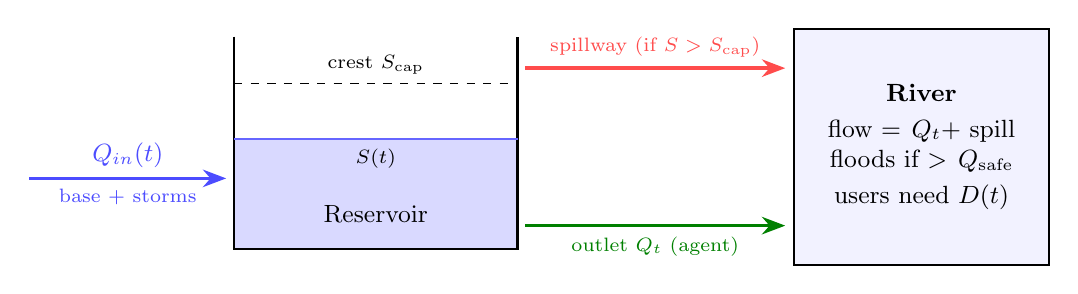
\begin{tikzpicture}[>=Stealth, font=\small]
  % reservoir
  \fill[blue!15] (0,0) rectangle (3.6,1.4);
  \draw[thick] (0,2.7) -- (0,0) -- (3.6,0) -- (3.6,2.7);
  \draw[dashed] (0,2.1) -- (3.6,2.1);
  \node[font=\scriptsize, above] at (1.8,2.1) {crest $\Scap$};
  \draw[blue!60, thick] (0,1.4) -- (3.6,1.4);
  \node[font=\scriptsize, below] at (1.8,1.4) {$S(t)$};
  \node at (1.8,0.45) {Reservoir};
  % inflow
  \draw[->, very thick, blue!70] (-2.6,0.9) -- node[above]{$Q_{in}(t)$} node[below, font=\scriptsize]{base + storms} (-0.1,0.9);
  % structures
  \draw[->, very thick, red!70] (3.7,2.3) -- node[above, font=\scriptsize]{spillway (if $S>\Scap$)} (7.0,2.3);
  \draw[->, very thick, green!50!black] (3.7,0.3) -- node[below, font=\scriptsize]{outlet $Q_t$ (agent)} (7.0,0.3);
  % river
  \node[draw, thick, fill=blue!5, minimum height=3cm, text width=3cm, align=center, anchor=west, font=\small]
    at (7.1,1.3) {\textbf{River}\\[2pt] flow $=Q_t+$ spill\\ floods if $>\Qsafe$\\[2pt] users need $D(t)$};
\end{tikzpicture}
\caption{The toy reservoir system.}
\label{fig:schematic}
\end{figure}

\subsection{Stochastic forcing}
For every episode (a 90-day season) the environment draws a new inflow
series on a 0.05-day grid:
\begin{align}
Q_{in}(t) &= \beta\,q_b + \sum_{j} h_j(t), \qquad \beta\sim U(0.7,1.3),\; q_b = 600~\text{m}^3/\text{d},\\
h_j(t) &= P_j\begin{cases} \tau/t_r & 0\le\tau<t_r\\ e^{-k_j(\tau-t_r)} & \tau\ge t_r\end{cases},\quad \tau=t-t_j,
\end{align}
with storm onsets $t_j$ arriving with probability $0.06$ per day, peaks
$P_j\sim U(5000,15000)$~m$^3$/d, rise time $t_r=0.5$~d and recession
constants $k_j\sim U(0.3,0.7)$~d$^{-1}$. The demand is
$D(t)=\bar D\,[1+0.3\sin(2\pi t/T+\psi)]$ with a random phase $\psi\sim U(0,2\pi)$. The
agent also receives a noisy forecast of the daily-mean inflow for the next
1, 2 and 3 days, with multiplicative log-normal errors that grow with lead
time ($\sigma_F=0.2\sqrt{k}$ for lead $k$ days). Figure~\ref{fig:forcing} shows
three realizations.

\begin{figure}[h]
\centering
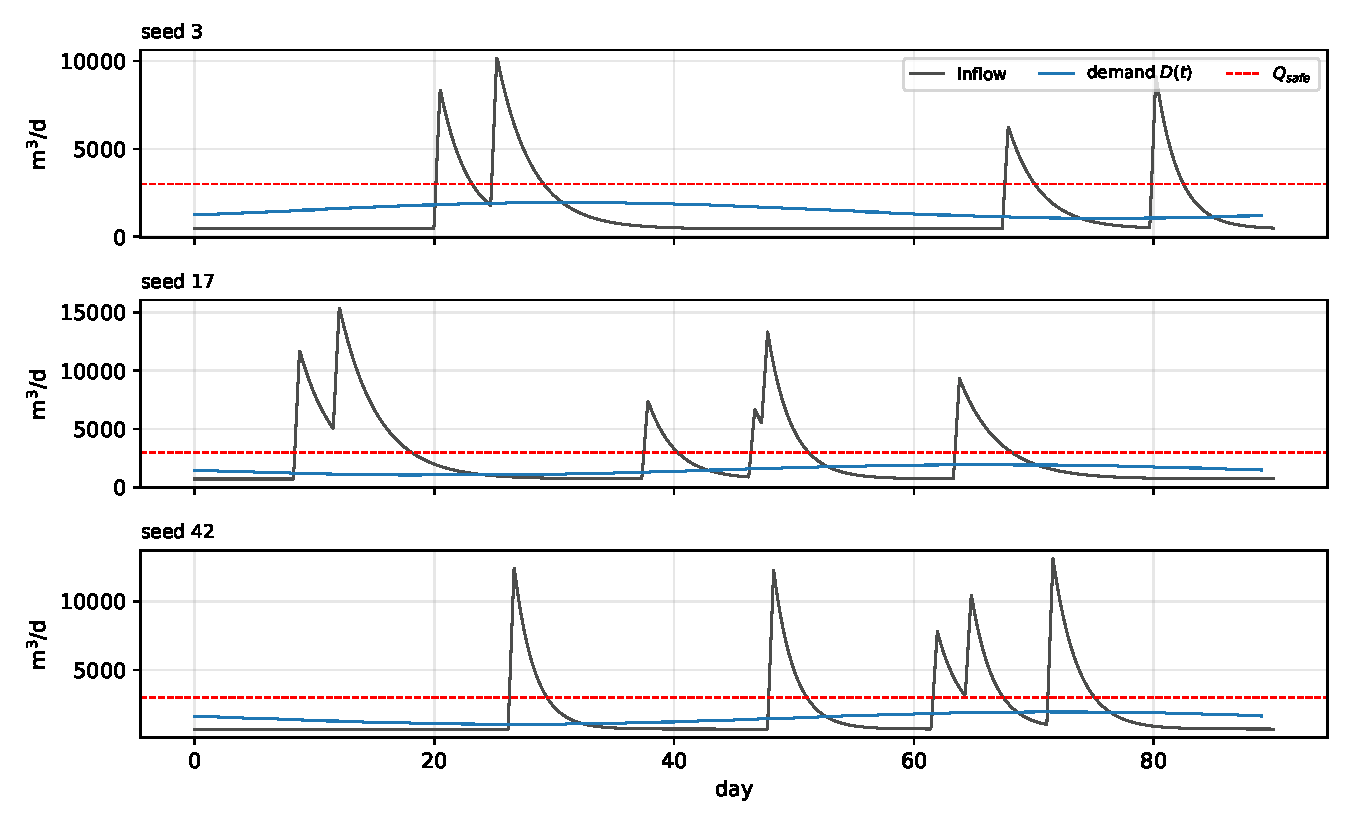
\includegraphics[width=0.9\textwidth]{figures/forcing_examples.pdf}
\caption{Three random forcing realizations (inflow, demand and the safe
channel capacity).}
\label{fig:forcing}
\end{figure}

\subsection{MDP formulation}\label{sec:mdp}
\begin{description}\itemsep2pt
\item[Decision step:] one day; episode length $T=90$ steps ($t=0,\dots,T-1$). The initial storage is drawn from $U(0.3,0.8)\,\Scap$.
\item[Observation] ($7$-dim, normalized):
\[o_t=\big(S_t/\Scap,\; Q_{in}(t)/\Qsafe,\; \hat F_{t+1}/\Qsafe,\; \hat F_{t+2}/\Qsafe,\; \hat F_{t+3}/\Qsafe,\; D_t/\Qsafe,\; 1-t/90\big),\]
where $\hat F_{t+k}$ is the $k$-day-ahead forecast of the daily-mean inflow.
\item[Action:] $a_t\in[-1,1]$, mapped to the target release $Q_t=\tfrac12(a_t+1)\,Q_{\mathrm{out}}$.
\item[Transition:] one-day OHQ simulation (Section~\ref{sec:ohqmodel}).
\item[Reward:] with $V^{rel}_t$ and $V^{sp}_t$ the released and spilled volumes over the day,
\begin{equation}
r_t = -\Big(\frac{\max(0,D_t-V^{rel}_t)}{D_t}\Big)^2
      - w_f\,\frac{\max(0,V^{rel}_t+V^{sp}_t-\Qsafe)}{\Qsafe}
      - w_s\,\frac{V^{sp}_t}{\Qsafe},
\end{equation}
with $w_f=2$ and $w_s=1$. At the end of the season a terminal penalty
$r_T^{\mathrm{term}}=-w_T\max(0,\,0.5\Scap-S_T)/\Scap$ ($w_T=5$) discourages emptying the
reservoir to avoid all flood risk.
\end{description}
\subsection{The objective function}\label{sec:objective}
Let $\xi$ denote everything random in a season: the storm onsets, peaks and
recessions, the base-flow factor $\beta$, the demand phase $\psi$, the
forecast errors and the initial storage $S_0$. An operating policy $\pi$ maps
the observation $o_t$ to a release $Q_t$. The quantity we want to
\emph{maximize} is the expected season return
\begin{equation}
J(\pi) \;=\; \mathbb{E}_{\xi}\Big[\sum_{t=0}^{T-1} r_t \;+\; r_T^{\mathrm{term}}\Big],
\label{eq:objective}
\end{equation}
equivalently, we \emph{minimize} the expected season cost
\[
\mathbb{E}_{\xi}\Big[\sum_{t=0}^{T-1}\Big(\underbrace{\Big(\tfrac{\max(0,D_t-V^{rel}_t)}{D_t}\Big)^2}_{\text{supply deficit}}
 + \underbrace{w_f\,\tfrac{\max(0,V^{rel}_t+V^{sp}_t-\Qsafe)}{\Qsafe}}_{\text{downstream flooding}}
 + \underbrace{w_s\,\tfrac{V^{sp}_t}{\Qsafe}}_{\text{uncontrolled spill}}\Big)
 + \underbrace{w_T\,\tfrac{\max(0,\,0.5\Scap-S_T)}{\Scap}}_{\text{end-of-season storage}}\Big],
\]
subject to the reservoir dynamics simulated by OHQ,
$S_{t+1}=S_t+V^{in}_t-V^{rel}_t-V^{sp}_t$, the outlet and spillway rules of
Section~\ref{sec:ohqmodel}, and $0\le Q_t\le Q_{\mathrm{out}}$. All terms
are dimensionless, so the weights $w_f=2$, $w_s=1$, $w_T=5$ set the
trade-off: one day of flow 100\% above $\Qsafe$ costs as much as two days of
a total supply failure.

Two versions of this objective appear in the report:
\begin{itemize}
\item \textbf{Evaluation} (Section~\ref{sec:results}) uses
Eq.~\eqref{eq:objective} directly: the undiscounted return of each test
season, averaged over 30 held-out seasons. This is the ``return'' in all
tables and plots.
\item \textbf{Training.} PPO maximizes the \emph{discounted} return
$J_\gamma(\pi_\theta)=\mathbb{E}\big[\sum_t \gamma^t r_t\big]$ with
$\gamma=0.99$, through the clipped surrogate $L(\theta)$ of
Section~\ref{sec:ppo}. Over a 90-day season, $\gamma^{89}\approx0.41$, so the
training objective weights late-season penalties, including the terminal
storage term, at roughly half their evaluation weight. This is a standard
variance-reduction compromise. It may explain part of the late-season
over-drawdown seen in Figure~\ref{fig:traj_med}; training with $\gamma$
closer to 1 is a cheap thing to try.
\end{itemize}
The baselines are not optimized by PPO: the tuned rule curve maximizes the
same Eq.~\eqref{eq:objective} by a one-dimensional grid search over its
threshold $\eta$.

The trade-off is the classic one: a full reservoir secures supply but leaves
no room to absorb storms, while an empty one does the opposite. The release
needed to make room is itself limited by $\Qsafe$, so the agent must
pre-release \emph{before} a forecast storm arrives.

%=====================================================================
\section{Building the OHQ model from Python}\label{sec:ohqmodel}
%=====================================================================

\subsection{Python bindings}
The bindings (\path{OpenHydroQual/PythonBindings/bindings.cpp}) expose
\code{System} with methods for loading templates, setting system values,
creating blocks and links, \code{finalize}, \code{solve} and
\code{write\_outputs}. There is no in-memory accessor for output time
series, so results are read back from the output file. Each worker
therefore uses its own working folder.

\subsection{Components}
The model uses existing OHQ templates:
\begin{center}
\small
\begin{tabular}{llp{5.2cm}}
\toprule
OHQ object & type (template) & role \\
\midrule
\code{Reservoir} & \code{Reservoir} & storage $S$, inflow time series (\code{Reservoir\_operation.json}) \\
\code{River} & \code{fixed\_head} & sink; its storage counts the released volume (\code{main\_components.json}) \\
\code{SpillSink} & \code{fixed\_head} & sink; its storage counts the spilled volume \\
\code{outlet} & \code{Reservoir\_link\_rule} & controlled release \\
\code{spillway} & \code{Reservoir\_link\_rule} & emergency overflow \\
\bottomrule
\end{tabular}
\end{center}

\code{Reservoir\_link\_rule} computes its flow from a piecewise-linear rule
in storage:
\begin{equation}
Q(S) = \begin{cases} Q_{\min} & S < S_{\min}\\
Q_{\min} + \frac{S-S_{\min}}{S_{\max}-S_{\min}}(Q_{\max}-Q_{\min}) & S_{\min}\le S\le S_{\max}\\
Q_{\max} & S > S_{\max}\end{cases}
\end{equation}
We use the same link type for both structures:
\begin{itemize}
\item \textbf{outlet:} $Q_{\min}=0$, $Q_{\max}=Q_t$ (the agent's action),
$S_{\min}=0$, $S_{\max}=S_{dead}=200$~m$^3$. The outlet releases exactly
$Q_t$ unless the reservoir is nearly empty, where the release tapers to
zero, so storage can never become negative.
\item \textbf{spillway:} $Q_{\min}=0$, $S_{\min}=\Scap$,
$S_{\max}=1.05\Scap$, $Q_{\max}=50{,}000$~m$^3$/d, which acts as an overflow
weir. An earlier, steeper ramp ($1.02\Scap$, $2\times10^5$~m$^3$/d) made
the Newton solver fail to converge when the spill switched off, so the
ramp was softened.
\end{itemize}

\subsection{One control interval}
Because the bindings do not expose a way to change a block's state on a
live \code{System}, the backend rebuilds the model for every decision step,
using the current storage as the initial condition. The inflow file holds
the whole season in absolute time, and each step simulates
$[t_0,t_0+1]$:

\begin{lstlisting}[language=Python]
s = ohq.System(); s.set_default_template_path(R); s.set_working_folder(W)
s.load_template(R + "main_components.json")
s.add_template(R + "Reservoir_operation.json")
for k, v in {"simulation_start_time": t0, "simulation_end_time": t0 + 1,
             "initial_time_step": 0.05, "max_timestep_increase_factor": 1,
             "n_threads": 1, "alloutputfile": W + "output.txt"}.items():
    s.set_system_value(k, str(v))
s.create_block("Reservoir", "Reservoir", {"Storage": S0, "inflow": inflow_file})
s.create_block("River", "fixed_head", {"head": "0", "Storage": "0"})
s.create_block("SpillSink", "fixed_head", {"head": "0", "Storage": "0"})
s.create_link("outlet", "Reservoir_link_rule", "Reservoir", "River",
              {"Q_min": 0, "Q_max": Q, "S_min": 0, "S_max": S_dead})
s.create_link("spillway", "Reservoir_link_rule", "Reservoir", "SpillSink",
              {"Q_min": 0, "Q_max": 5e4, "S_min": S_cap, "S_max": 1.05 * S_cap})
s.finalize(); s.solve(True, False); s.write_outputs()
# read S(t0+1), River storage (= released volume), SpillSink storage (= spill)
\end{lstlisting}
(Numbers are converted to strings in the actual code.) Two practical notes:
\code{set\_system\_value} returned \code{False} even when the setting was
applied (fixed in OHQ, see the last section), and the \code{Reservoir\_link\_rule} template stores its
\code{"unit"} entry inside the \code{rule} dictionary, so OHQ prints
harmless \emph{``property `ft' does not exist''} messages.

%=====================================================================
\section{Verifying the simulator output}
%=====================================================================

Before using OHQ inside an RL loop we checked it against a case with an
analytical solution: constant inflow $1000$~m$^3$/d, release
$150$~m$^3$/d and $S_0=1000$~m$^3$, so that $S(t)=1000+850\,t$.

\subsection{Finding: one-step time-stamp lag}
The first test runs disagreed with the analytical solution, and the error
grew with the time step. Reading \code{System::Solve} showed two causes:
\begin{enumerate}
\item The time loop runs \code{while (t < tend + dt)}, so the last step
overshoots $t_{end}$. With the default adaptive step (allowed to grow to
$50\times$ the initial step), this overshoot can be large.
\item The current OHQ source stamps each output row with the time at the
\emph{end} of the step (\code{PopulateOutputs(true, t + dt)}), and a code
comment notes this was changed. The compiled \code{libOHQLib.so} the
bindings link against predates the change and stamps the row with the
\emph{start} time of the step. Each row therefore holds the state one step
later than its label says.
\end{enumerate}

Figure~\ref{fig:stamping} shows the storage error relative to the
analytical solution. With the step held fixed, reassigning each row the
next row's stamp makes the error exactly zero. With the default growing
step, the error stays offset even after this correction. The environment
therefore (i) fixes the step (\code{max\_timestep\_increase\_factor = 1}),
(ii) reassigns each row the next row's stamp and interpolates at
$t_0+1$, and (iii) detects automatically at start-up which convention the
linked library uses, by running this analytical test. The environment
keeps working if OHQLib is rebuilt with the corrected stamping.

\paragraph{Update (rebuilt library).} After rebuilding \code{libOHQLib}
(v2.1.1) and the bindings from the current source, the self-check selects
the end-of-step convention. The output now matches the analytical solution
exactly with both the fixed and the default growing step, and the first
row holds the true initial state. The overshoot past $t_{end}$ remains by
design: with the growing step, the 1-day run above ended at $t=1.8$, so up
to 80\% extra time was simulated. The environment therefore keeps the
step fixed. Training results are unaffected, since the physics is
identical (same episode return, to 4 decimals). Per-step cost dropped from
about 5.1 to 4.0~ms.

\begin{figure}[h]
\centering
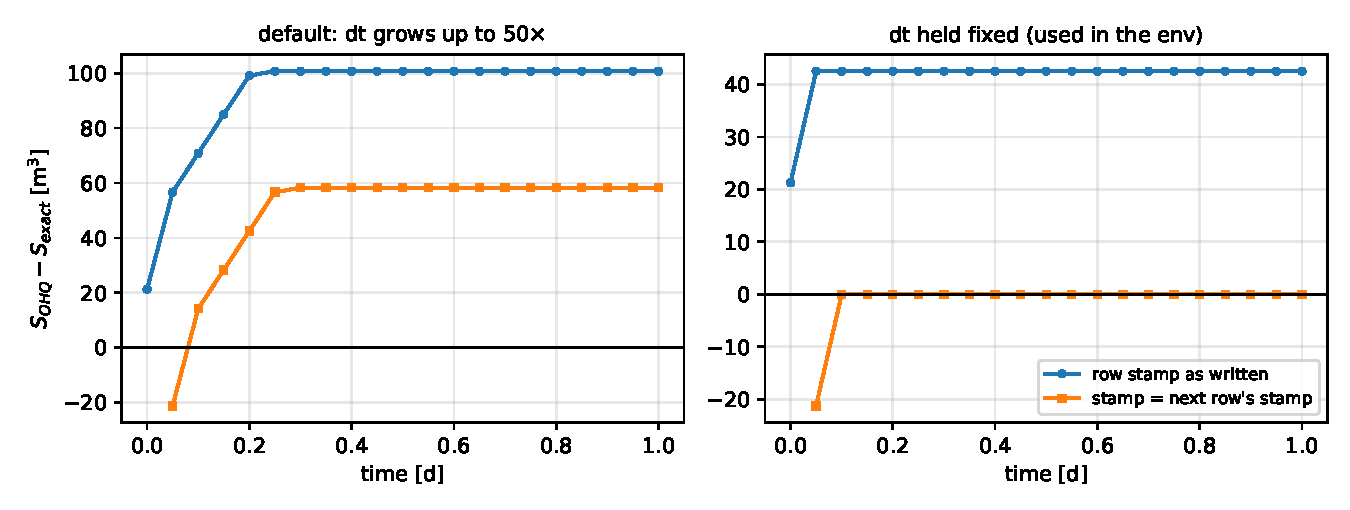
\includegraphics[width=0.95\textwidth]{figures/stamping_check.pdf}
\caption{Error of the OHQ storage relative to the analytical solution for
a one-day run (initial step 0.05~d). Left: default adaptive step. Right:
fixed step, as used in the environment. Assigning each row the next row's
stamp removes the error (after the very first row).}
\label{fig:stamping}
\end{figure}

\subsection{Episode mass balance}
Over a full episode, run with the rule-curve policy, we compare the daily
change in storage with the exact inflow volume (trapezoidal integral of
the forcing) minus the released and spilled volumes
(Figure~\ref{fig:massbalance}). The residual follows a characteristic
$+/-$ pattern on storm days: positive on the rising limb, then negative and
decaying. This is consistent with OHQ evaluating the piecewise-linear
inflow series slightly offset within the implicit step, and it is a
property of the time discretization, not of the bookkeeping. The residual
integrates to nearly zero: the largest daily residual is 231~m$^3$, while the cumulative residual over the season is 9.3~m$^3$ out of 189{,}339~m$^3$ of inflow (0.005\%).


\begin{figure}[h]
\centering
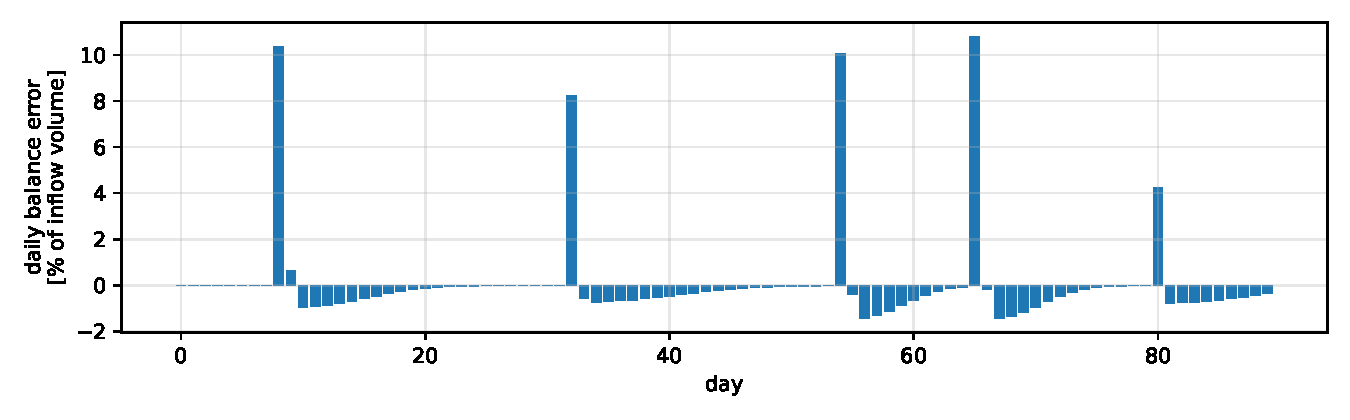
\includegraphics[width=0.95\textwidth]{figures/mass_balance.pdf}
\caption{Daily mass-balance residual
$S_t+V^{in}_t-V^{rel}_t-V^{sp}_t-S_{t+1}$ as a percentage of the day's
inflow volume.}
\label{fig:massbalance}
\end{figure}

%=====================================================================
\section{The RL algorithm (PPO)}\label{sec:ppo}
%=====================================================================

We use \emph{Proximal Policy Optimization} (PPO) \cite{schulman2017ppo},
one of the most widely used RL algorithms. It is an actor--critic method
built directly on the policy gradient of Eq.~\eqref{eq:pg}. It is
implemented from scratch in about 150 lines of PyTorch
(\code{train\_ppo.py}), so every step below can be traced in the code.

\subsection{The idea}
PPO repeats one cycle:
\begin{enumerate}\itemsep1pt
\item \textbf{Collect experience.} Run the current policy (with its
exploration noise) in the simulator for a while and record every
$(o_t,a_t,r_t)$.
\item \textbf{Score each decision.} Use the critic to estimate each
action's advantage: was it better or worse than expected?
\item \textbf{Improve the policy, carefully.} Change $\theta$ to make
good actions more likely and bad ones less likely, \emph{but not by too
much in one go}.
\item \textbf{Improve the critic.} Fit $V_\phi$ to the returns just
observed, so the next round's advantage estimates are better.
\end{enumerate}
The phrase ``not by too much'' is what distinguishes PPO. A policy-gradient
step uses data collected with the \emph{old} policy, so it is only
trustworthy for policies close to it. A large step can jump to a policy
that behaves very differently, where the old data say nothing, and
performance can collapse. Engineers will recognize the same concern behind
step-size control in Newton's method or the damping term in
Levenberg--Marquardt: trust the local model only within a limited region.

\subsection{The networks}
Two separate small networks are used. Each has two hidden layers of 64
units with $\tanh$ activations.
\begin{itemize}\itemsep1pt
\item \textbf{Actor:} $o_t\mapsto\mu_\theta(o_t)$, the mean of the action.
The action is drawn as $a_t\sim\mathcal N(\mu_\theta(o_t),\sigma^2)$. The
spread $\sigma$ is one more learned parameter, initialized at
$e^{-0.5}\approx0.6$ (on an action range of $[-1,1]$, so exploration starts
wide). The environment clips the action to $[-1,1]$ and maps it to a
release.
\item \textbf{Critic:} $o_t\mapsto V_\phi(o_t)$, the predicted
(discounted) return still to come.
\end{itemize}
For evaluation, the trained actor is used deterministically:
$a_t=\mathrm{clip}(\mu_\theta(o_t))$.

\subsection{Step 2 in detail: generalized advantage estimation}
The TD error of Eq.~\eqref{eq:td} is a one-day look-ahead. It has low
variance, but it is biased when the critic is wrong. The full remaining
return is unbiased but noisy. \emph{Generalized advantage estimation} (GAE)
\cite{schulman2016gae} blends all look-ahead lengths with a geometric
weight $\lambda\in[0,1]$:
\begin{equation}
\hat A_t=\sum_{l\ge0}(\gamma\lambda)^l\,\delta_{t+l},\qquad
\delta_t=r_t+\gamma V_\phi(o_{t+1})(1-d_t)-V_\phi(o_t),
\label{eq:gae}
\end{equation}
where $d_t=1$ on the last day of a season (there is no ``tomorrow'' to
bootstrap from). $\lambda=0$ gives the one-day TD error. $\lambda=1$ gives
the full remaining return minus the critic's prediction. We use
$\lambda=0.95$, so credit for a flood is spread back over roughly the
previous $1/(1-\gamma\lambda)\approx17$ days. The sum is computed in one
backward pass over the recorded data. The critic's regression target is
$\hat R_t=\hat A_t+V_\phi(o_t)$. Before each update the advantages are
standardized (zero mean, unit variance), which only rescales the step.

\subsection{Step 3 in detail: the clipped objective}
After the data are collected, the policy used to collect them is frozen as
$\pi_{\theta_{old}}$. For a candidate $\theta$, the \emph{probability
ratio}
\[
\rho_t(\theta)=\frac{\pi_\theta(a_t\mid o_t)}{\pi_{\theta_{old}}(a_t\mid o_t)}
\]
says how much more (or less) likely the new policy is to take the recorded
action. The objective $\mathbb E[\rho_t\hat A_t]$ has the same gradient as
Eq.~\eqref{eq:pg} at $\theta=\theta_{old}$, and it can be maximized with
several gradient steps on the same data. Left alone, though, it would keep
pushing $\rho_t$ for good actions towards infinity. PPO therefore
maximizes the \emph{clipped} objective
\begin{equation}
L^{\mathrm{clip}}(\theta)=\mathbb E_t\Big[\min\big(\rho_t\hat A_t,\;\mathrm{clip}(\rho_t,\,1-\epsilon,\,1+\epsilon)\,\hat A_t\big)\Big],\qquad \epsilon=0.2 .
\label{eq:clip}
\end{equation}
Two cases make it concrete. If $\hat A_t>0$ (a good action), the objective
grows with $\rho_t$ until $\rho_t=1.2$ and is flat beyond, so there is no
incentive to make that action more than 20\% more likely in one round. If
$\hat A_t<0$ (a bad action), the objective improves as $\rho_t$ falls, but
only until $\rho_t=0.8$. The $\min$ makes sure clipping can only remove
incentives, never add them. The result is a cheap, approximate trust
region.

The quantity actually minimized by gradient descent combines the actor and
critic losses:
\begin{equation}
L(\theta,\phi)=-L^{\mathrm{clip}}(\theta)+c_v\,\tfrac12\,\mathbb E_t\big[(V_\phi(o_t)-\hat R_t)^2\big],\qquad c_v=0.5 .
\label{eq:ppo_loss}
\end{equation}
The first term improves the policy and the second fits the critic by least
squares.

\subsection{The full training loop}
\begin{center}
\fbox{\begin{minipage}{0.92\textwidth}
\small
\textbf{PPO as implemented in \code{train\_ppo.py}}
\begin{enumerate}\itemsep1pt
\item Initialize actor $\theta$, critic $\phi$, $\log\sigma=-0.5$. Start 16 simulators, each with its own random season.
\item Repeat for 100 updates (single reservoir) or 245 updates (cascade):
\begin{enumerate}\itemsep0pt
\item \emph{Rollout:} each simulator runs 256 days with the current stochastic policy, so 4{,}096 $(o,a,r)$ records per update. A finished season immediately restarts with a new random season.
\item \emph{Advantages:} compute $\delta_t$, $\hat A_t$ (Eq.~\ref{eq:gae}) and $\hat R_t$ for every record; standardize $\hat A_t$.
\item \emph{Optimize:} 10 passes (epochs) over the 4{,}096 records in shuffled minibatches of 256; on each minibatch take one Adam gradient step on $L(\theta,\phi)$ (Eq.~\ref{eq:ppo_loss}), with gradient norm clipped at 0.5.
\end{enumerate}
\item Save $\theta$ (the trained policy).
\end{enumerate}
\end{minipage}}
\end{center}

\subsection{Hyperparameters and what they control}
\begin{center}
\small
\begin{tabular}{lrp{0.55\textwidth}}
\toprule
setting & value & what it controls\\
\midrule
parallel simulators & 16 & throughput; one OHQ instance per CPU worker\\
rollout length & 256 days & experience collected per simulator per update\\
samples per update & 4{,}096 & size of the batch the policy learns from each round\\
epochs per update & 10 & how many times each batch is reused\\
minibatch size & 256 & records per gradient step\\
learning rate (Adam) & $3\times10^{-4}$ & gradient step size\\
discount $\gamma$ & 0.99 & how far ahead the agent looks (effective horizon $\sim1/(1-\gamma)=100$ days)\\
GAE $\lambda$ & 0.95 & bias--variance trade-off of the advantage estimate\\
clip $\epsilon$ & 0.2 & maximum change in action probabilities per round (trust region)\\
value coefficient $c_v$ & 0.5 & weight of the critic's loss\\
gradient-norm clip & 0.5 & guards against occasional huge gradients\\
total steps & 409{,}600 / $\sim10^6$ & training budget, single reservoir / cascade\\
\bottomrule
\end{tabular}
\end{center}
These are standard PPO defaults. None were tuned for this problem.

\paragraph{Parallel rollouts.} The 16 simulators run in separate processes
(\path{gymnasium.vector.AsyncVectorEnv}). Each owns its own OHQ instance
and working folder. When a season ends, Gymnasium restarts it one step
later and returns one dummy record, which is masked out of the update.

\paragraph{A performance pitfall.} The first parallel run made almost no
progress. Every worker sat at $\approx370\%$ CPU because OHQ's solver
defaults to \code{n\_threads = 8} (OpenMP), and BLAS/PyTorch add their own
threads. Sixteen workers times eight threads oversubscribed the 32-core
machine. Whenever OHQ models run in parallel, \code{n\_threads} must be 1.
With \code{n\_threads = 1} in OHQ and \code{OMP\_NUM\_THREADS = 1} /
\code{torch.set\_num\_threads(1)} in the workers, throughput rose to
$\approx1{,}200$ environment steps per second.



%=====================================================================
\section{Results for the single reservoir}\label{sec:results}
%=====================================================================

\subsection{How we judge a policy}
A learned policy is only useful if it performs well on seasons it has
never seen. The procedure, used throughout, is:
\begin{itemize}\itemsep1pt
\item \textbf{Held-out test seasons.} Thirty seasons generated from seeds
that were never used in training (seeds $10{,}000$--$10{,}029$). Every
policy faces exactly the same 30 storm sequences.
\item \textbf{Score.} The season return of Eq.~\eqref{eq:objective}:
minus the total penalty, so 0 is perfect and higher is better. We also
report its components (supply, flood, spill, terminal).
\item \textbf{Paired comparison.} Some seasons are much stormier than
others, so the spread of returns across seasons is large for \emph{every}
policy. Comparing means alone mixes up policy quality with weather luck.
Because all policies see the same seasons, we instead compute, season by
season, the difference in return between PPO and a baseline. We report its
mean and its standard error (standard deviation over $\sqrt{30}$). A mean
difference larger than about twice its standard error is unlikely to be
luck. We also count in how many of the 30 seasons PPO did better.
\item \textbf{Fair baselines.} A comparison is only as good as its
opponent, so the rule curve's parameter is tuned on a separate set of
seasons before testing.
\end{itemize}

\subsection{Training}
Training used 409{,}600 environment steps (100 PPO updates, about 4{,}500
episodes), which took about 5 minutes with 16 workers at
$\approx1{,}450$ steps/s. Each step is one complete OHQ model build and solve,
so this is also about $4\times10^5$ OHQ runs.
Figure~\ref{fig:learning} shows that the mean return rises from about $-52$
(a near-random policy) to about $-20$ within the first $\sim$150k steps and
then plateaus. The exploration standard deviation keeps shrinking
($0.59\to0.15$). The remaining noise in the curve comes from the
storm-to-storm variability of the episodes, not from the policy: a season
with five large storms costs far more under \emph{any} policy than a dry
one.


\begin{figure}[h]
\centering
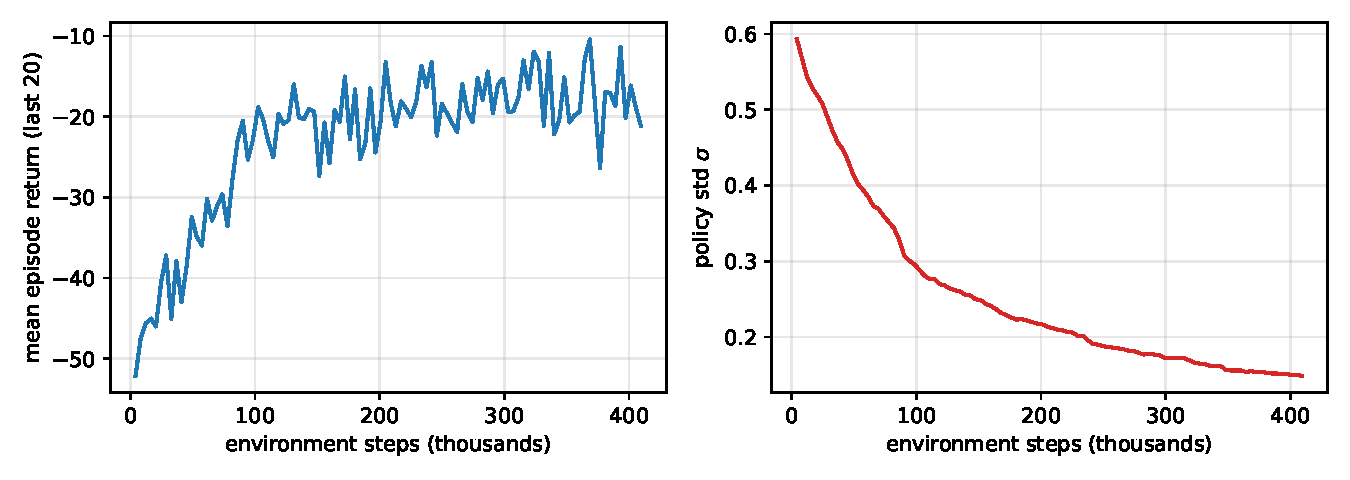
\includegraphics[width=0.95\textwidth]{figures/learning_curve.pdf}
\caption{Left: mean return of the last 20 completed training episodes.
Right: the policy's exploration standard deviation.}
\label{fig:learning}
\end{figure}

\subsection{Comparison with baselines}
We evaluate three policies on the same 30 held-out storm sequences
(seeds $10{,}000$--$10{,}029$, never seen in training):
\begin{description}\itemsep2pt
\item[Demand only:] release $Q_t=D_t$.
\item[Rule curve (0.8):] a standard operating policy with a flood rule:
release $D_t$, and above $\eta\Scap$ also release the excess storage over
one day: $Q_t=\min\big(\Qsafe,\,D_t+(S_t-\eta\Scap)/\Delta t\big)$ with
$\Delta t=1$~d, and $\eta=0.8$.
\item[Tuned rule:] the same rule with $\eta$ tuned by grid search on
separate seeds (see below).
\item[PPO:] the trained agent (deterministic).
\end{description}

\begin{table}[h]
\centering
\small
\begin{tabular}{lrrrrrrr}
\toprule
Policy & Return & Supply & Flood & Spill & Terminal & Deficit [\%] & Flood days \\
\midrule
Demand only & $-38.41\pm35.47$ & -1.24 & -20.39 & -16.33 & -0.43 & 2.2 & 9.3 \\
Rule curve (0.8) & $-22.56\pm26.30$ & -1.31 & -13.76 & -6.88 & -0.61 & 2.3 & 6.9 \\
Tuned rule (0.4) & $-15.81\pm23.95$ & -2.95 & -7.73 & -3.87 & -1.25 & 5.6 & 3.5 \\
PPO & $-15.01\pm23.38$ & -2.88 & -7.50 & -3.39 & -1.24 & 6.0 & 6.6 \\
\bottomrule
\end{tabular}

\caption{Mean over 30 test episodes. The return is split into its supply,
flood, spill and terminal components (all penalties, so higher is better).
\emph{Deficit} is the fraction of total demand not delivered. \emph{Flood
days} counts days with river flow above $\Qsafe$.}
\label{tab:results}
\end{table}

\paragraph{Tuning the baseline.} The 0.8 threshold of the rule curve was an
arbitrary first choice. To give the agent a fair opponent, we also
grid-searched the threshold on 30 separate \emph{tuning} seeds
($20{,}000$--$20{,}029$; Figure~\ref{fig:tuning}). The best value, a flood
rule that starts releasing above 0.4\,$\Scap$, is then
evaluated on the same test seeds as everything else (``Tuned rule'').

\begin{figure}[h]
\centering
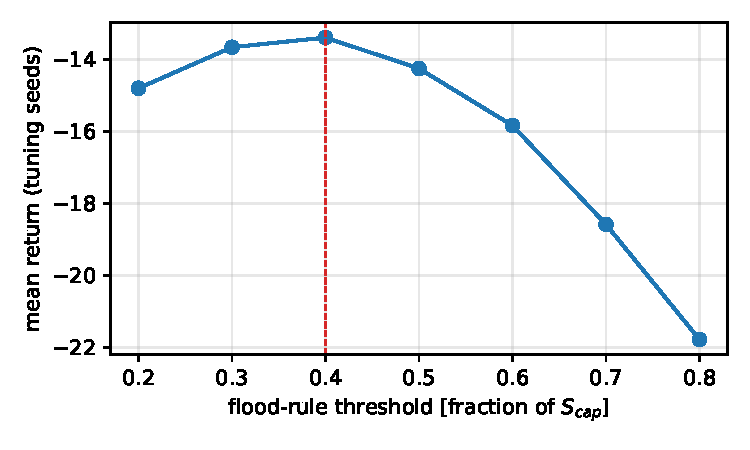
\includegraphics[width=0.5\textwidth]{figures/threshold_tuning.pdf}
\caption{Mean return of the rule curve versus its flood-rule threshold, on
the tuning seeds.}
\label{fig:tuning}
\end{figure}

\paragraph{Paired comparison.} Because every policy sees the same 30 storm
sequences, the fair test is the per-episode difference in return
(Table~\ref{tab:paired}). The spread in Table~\ref{tab:results} is
dominated by how stormy each season is, and this pairing cancels it.

\begin{table}[h]
\centering
\begin{tabular}{lrrr}
\toprule
baseline & mean(PPO $-$ baseline) & std.\ error & PPO better in \\
\midrule
Demand only & $+23.39$ & 4.01 & 23/30 \\
Rule curve (0.8) & $+7.54$ & 2.11 & 20/30 \\
Tuned rule (0.4) & $+0.79$ & 0.86 & 12/30 \\
\bottomrule
\end{tabular}

\caption{Paired differences in episode return, PPO minus baseline, on the
30 test episodes.}
\label{tab:paired}
\end{table}

\paragraph{What the agent learned.}
\begin{itemize}
\item PPO clearly beats releasing the demand only (by about 23 return
points) and the untuned rule curve (by about 7.5 points, better in 20 of 30
episodes). It cuts the flood penalty roughly in half and the spill penalty
by a factor of about two.
\item It does this with a \emph{drawdown hedging} strategy
(Figure~\ref{fig:traj_best}). PPO releases more than the demand most of the
time and keeps the reservoir low, so storms are absorbed instead of
spilled. The cost is a higher supply deficit (6\% versus 2\% of demand)
and occasional near-empty periods. The policy map
(Figure~\ref{fig:policymap}) shows the release increasing smoothly with
both storage and the forecast inflow.
\item Against the \emph{tuned} rule curve the difference is
$+0.8\pm0.9$, i.e.\ statistically indistinguishable. In effect, PPO
rediscovered ``keep the reservoir around 40\% full and release the
excess'', which is close to the best policy in the rule-curve family for
this reward. The two policies reach the same return differently: the tuned
rule floods on fewer days, while PPO exceeds $\Qsafe$ more often but by
smaller margins.
\end{itemize}

\paragraph{Interpretation.} For a single reservoir with a 3-day forecast
and this reward, a well-tuned one-parameter rule is already near-optimal.
RL earns its keep only when that stops being true, for example with
multiple interacting reservoirs, nonlinear water-quality objectives,
longer forecasts whose skill varies, or rewards that a fixed rule cannot
express. The value of this exercise is the pipeline: the same
environment-and-agent code applies unchanged to richer OHQ models.


\begin{figure}[h]
\centering
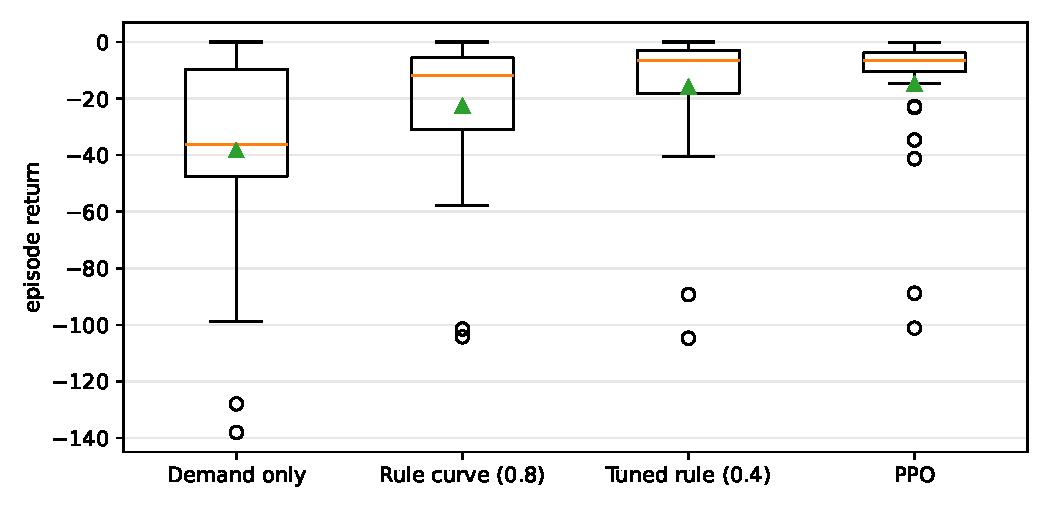
\includegraphics[width=0.7\textwidth]{figures/return_boxplot.pdf}
\caption{Distribution of test-episode returns.}
\label{fig:box}
\end{figure}

\begin{figure}[p]
\centering
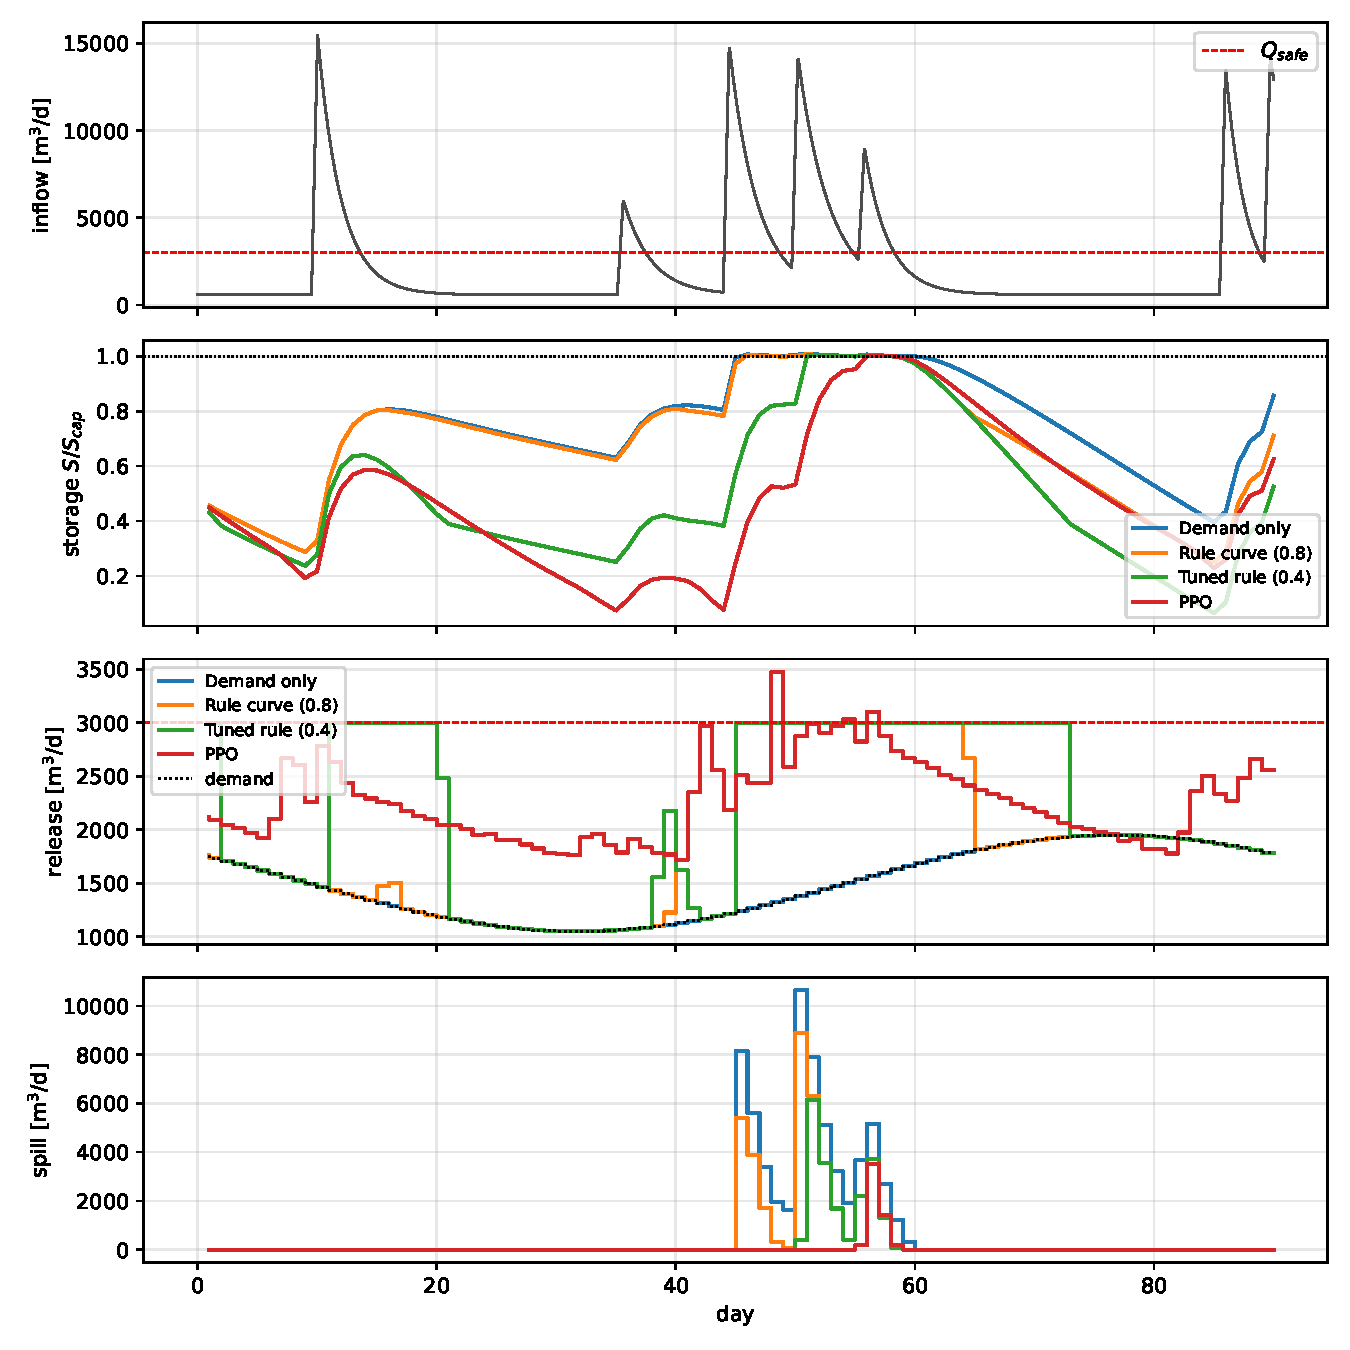
\includegraphics[width=0.95\textwidth]{figures/trajectory_best_gain.pdf}
\caption{Test episode with the largest PPO gain over the rule curve (0.8). From
top: inflow, storage, release (dotted: demand; dashed: $\Qsafe$), spill.}
\label{fig:traj_best}
\end{figure}

\begin{figure}[p]
\centering
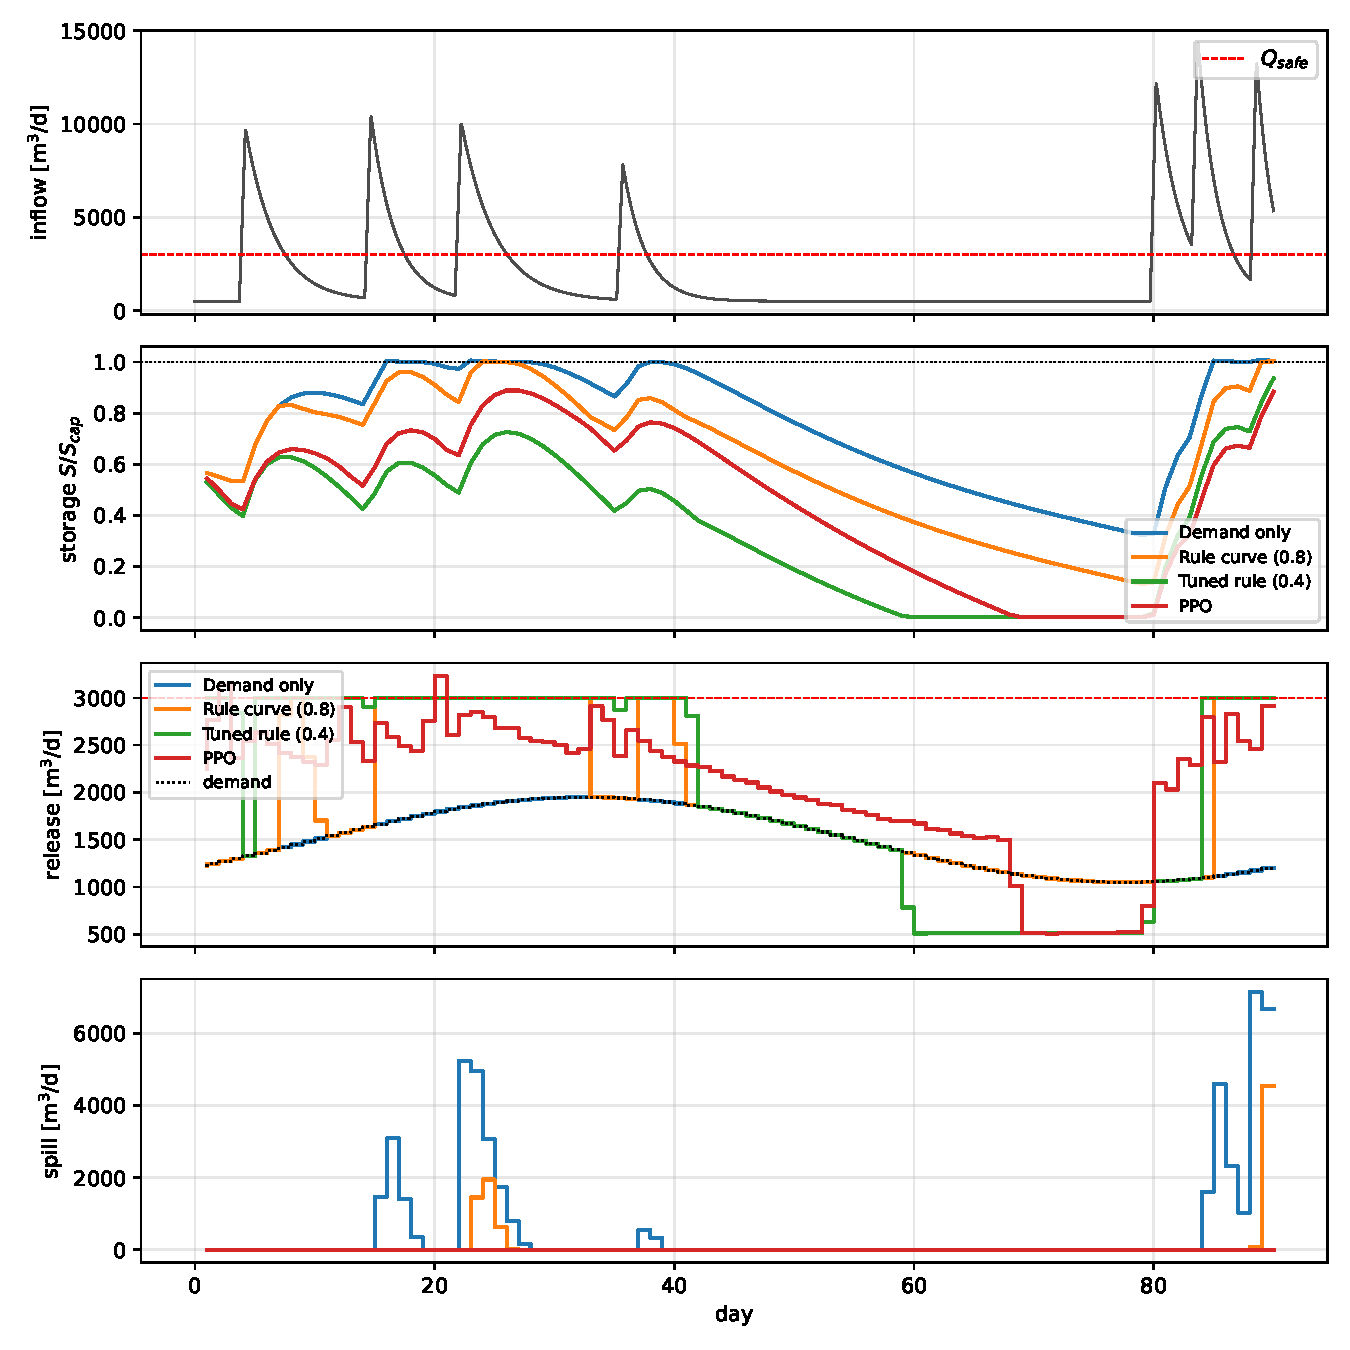
\includegraphics[width=0.95\textwidth]{figures/trajectory_median.pdf}
\caption{A test episode with the median PPO-vs-rule-curve (0.8) difference.}
\label{fig:traj_med}
\end{figure}

\begin{figure}[h]
\centering
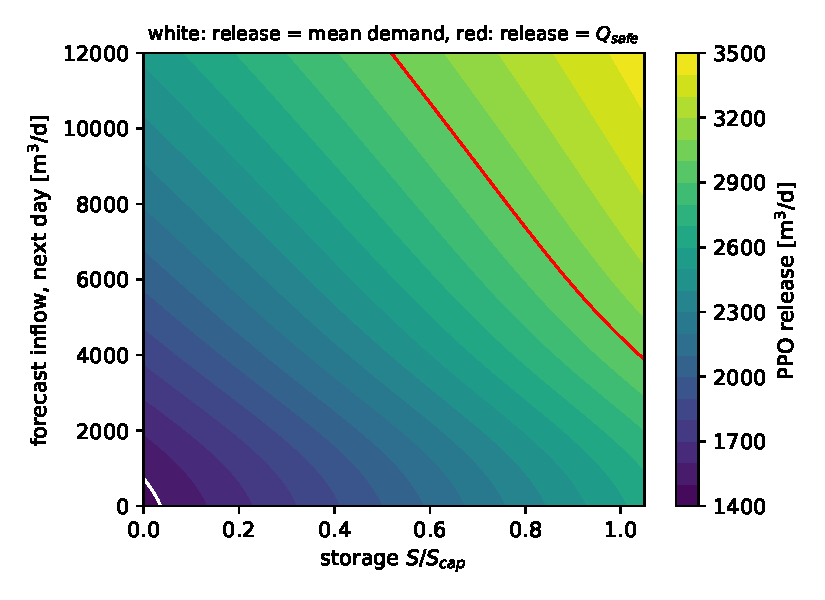
\includegraphics[width=0.6\textwidth]{figures/policy_map.pdf}
\caption{Learned release as a function of storage and the inflow forecast.
The current inflow and the 1- and 2-day forecasts are set to the value on the
vertical axis, the 3-day forecast to $0.6\times$ that value, with mean
demand at mid-season.}
\label{fig:policymap}
\end{figure}

%=====================================================================
\section{Performance and the case for a codegen backend}\label{sec:performance}
%=====================================================================

RL needs a very large number of short simulations; this run alone used
about $4\times10^5$ one-day OHQ solves. Figure~\ref{fig:timing} breaks
down the cost of one step.

\begin{figure}[h]
\centering
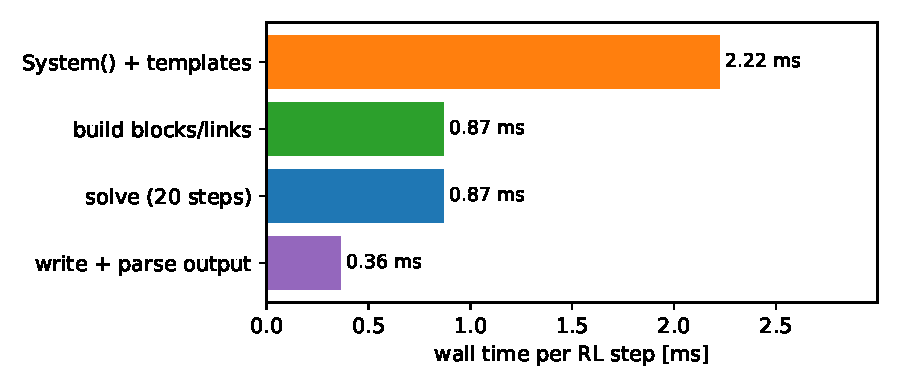
\includegraphics[width=0.75\textwidth]{figures/timing_breakdown.pdf}
\caption{Wall time per environment step for the interpreted OHQ backend
(mean of 50 steps, single thread).}
\label{fig:timing}
\end{figure}

One step costs about 4.3~ms, but the numerical solve (20 implicit steps of 0.05~d) accounts for only 0.9~ms. The remaining 3.5~ms (80\%) is overhead: constructing a \code{System} and parsing the JSON templates (2.2~ms), building blocks and links (0.9~ms), and writing and parsing the output file (0.4~ms). The overhead is a fixed per-step cost, independent of how hard the physics is. A codegen-compiled model that is built once and only has its state reset between steps would remove nearly all of it, giving roughly a 5$\times$ speed-up for this model even before any gain in the solver itself.


\begin{figure}[h]
\centering
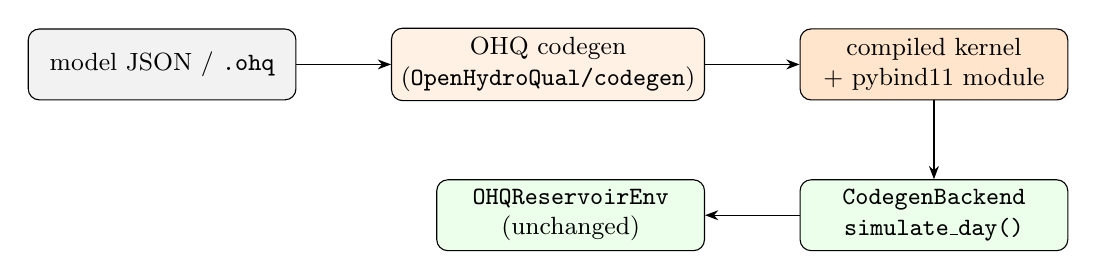
\begin{tikzpicture}[>=Stealth, font=\small,
  box/.style={draw, rounded corners, align=center, minimum height=0.9cm, fill=#1}, box/.default=white]
  \node[box=gray!10, minimum width=3.4cm] (a) {model JSON / \code{.ohq}};
  \node[box=orange!10, right=1.2cm of a, minimum width=3.4cm] (b) {OHQ codegen\\(\code{OpenHydroQual/codegen})};
  \node[box=orange!20, right=1.2cm of b, minimum width=3.4cm] (c) {compiled kernel\\+ pybind11 module};
  \node[box=green!8, below=1.0cm of c, minimum width=3.4cm] (d) {\code{CodegenBackend}\\\code{simulate\_day()}};
  \node[box=green!8, left=1.2cm of d, minimum width=3.4cm] (e) {\code{OHQReservoirEnv}\\(unchanged)};
  \draw[->] (a) -- (b); \draw[->] (b) -- (c); \draw[->] (c) -- (d); \draw[->] (d) -- (e);
\end{tikzpicture}
\caption{Planned replacement of the interpreted backend.}
\end{figure}

\paragraph{Backend contract.} Any replacement only needs to implement
\begin{lstlisting}[language=Python]
class Backend:
    def set_inflow(self, t, q): ...          # forcing for the whole episode
    def simulate_day(self, t0, S0, Q):       # one control interval
        return S1, released_volume, spilled_volume
    def close(self): ...
\end{lstlisting}
and is passed to the environment as \code{OHQReservoirEnv(backend=...)}.
A compiled kernel that keeps its state in memory between calls would also
remove the per-step file round trip and the template parsing, and would
allow batched, vectorized rollouts within a single process.

%=====================================================================
\section{A harder problem -- a two-reservoir cascade}\label{sec:cascade}
%=====================================================================

The single reservoir turned out to be easy enough that a tuned
one-parameter rule matched PPO. Here the agent operates two reservoirs in
series. An uncontrolled tributary joins below them, so the agent must
coordinate where to hold flood space and when to release.

\subsection{System}
\begin{figure}[h]
\centering
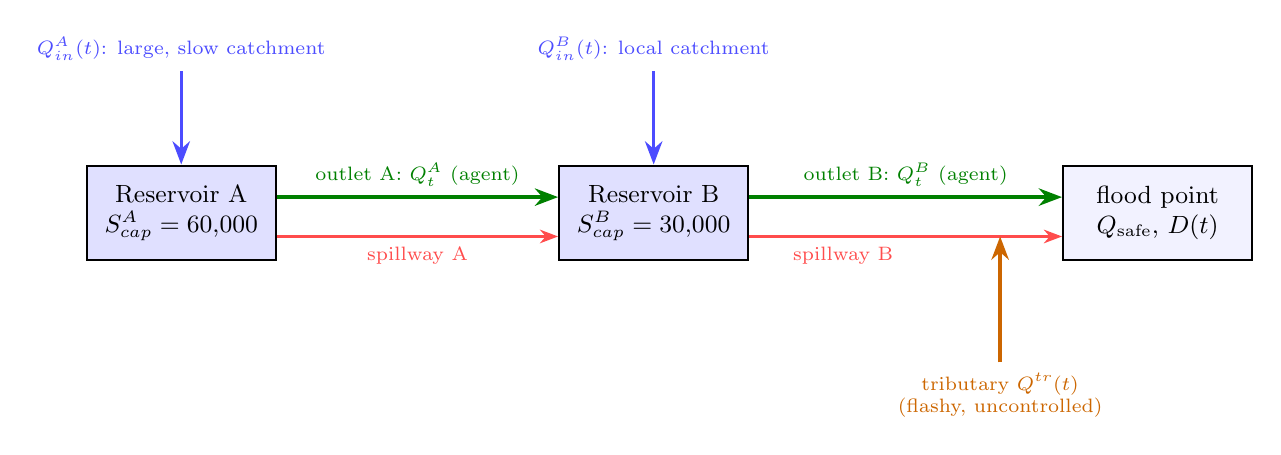
\begin{tikzpicture}[>=Stealth, font=\small,
  res/.style={draw, thick, fill=blue!12, minimum width=2.4cm, minimum height=1.2cm, align=center}]
  \node[res] (A) at (0,0) {Reservoir A\\$S^A_{cap}=60{,}000$};
  \node[res] (B) at (6,0) {Reservoir B\\$S^B_{cap}=30{,}000$};
  \node[draw, thick, fill=blue!5, minimum width=2.4cm, minimum height=1.2cm, align=center] (F) at (12.4,0) {flood point\\$\Qsafe$, $D(t)$};
  \draw[->, very thick, blue!70] (0,1.8) node[above, font=\scriptsize]{$Q^A_{in}(t)$: large, slow catchment} -- (A.north);
  \draw[->, very thick, blue!70] (6,1.8) node[above, font=\scriptsize]{$Q^B_{in}(t)$: local catchment} -- (B.north);
  \draw[->, very thick, green!50!black] ([yshift=2mm]A.east) -- node[above, font=\scriptsize]{outlet A: $Q^A_t$ (agent)} ([yshift=2mm]B.west);
  \draw[->, thick, red!70] ([yshift=-3mm]A.east) -- node[below, font=\scriptsize]{spillway A} ([yshift=-3mm]B.west);
  \draw[->, very thick, green!50!black] ([yshift=2mm]B.east) -- node[above, font=\scriptsize]{outlet B: $Q^B_t$ (agent)} ([yshift=2mm]F.west);
  \draw[->, thick, red!70] ([yshift=-3mm]B.east) -- node[below, font=\scriptsize, pos=0.3]{spillway B} ([yshift=-3mm]F.west);
  \draw[->, very thick, orange!80!black] (10.4,-1.9) node[below, font=\scriptsize, align=center]{tributary $Q^{tr}(t)$\\(flashy, uncontrolled)} -- (10.4,-0.3);
\end{tikzpicture}
\caption{The two-reservoir cascade. Reservoir A's outflow, through its
outlet or spillway, enters reservoir B. The flood point and the downstream
users sit below the tributary confluence.}
\label{fig:cascade_schematic}
\end{figure}

Storms are regional: every storm hits all three catchments, with each
catchment responding at its own scale and speed (all flows in m$^3$/d):
\begin{center}
\small
\begin{tabular}{lrrrrr}
\toprule
catchment & base flow & peak scale $\bar P$ & delay & rise time & recession $k$ [d$^{-1}$] \\
\midrule
A (upstream, large) & 500 & 5{,}000 & 0.5 d & 1.0 d & $U(0.2,0.4)$\\
B (local) & 200 & 3{,}000 & 0 & 0.5 d & $U(0.4,0.7)$\\
tributary & 300 & 4{,}000 & 0 & 0.25 d & $U(0.7,1.2)$\\
\bottomrule
\end{tabular}
\end{center}
Storm onsets arrive with probability 0.05 per day. Each storm has a common
intensity $m\sim U(0.5,1.5)$, and catchment $c$ gets peak
$\bar P_c\,m\,U(0.8,1.2)$ with the hydrograph shape of
Section~\ref{sec:objective}. All base flows share one factor
$\beta\sim U(0.7,1.3)$. The demand at the flood point has mean
$\bar D=2{,}000$~m$^3$/d with a $\pm30\%$ seasonal swing. The river's safe
capacity is $\Qsafe=4{,}000$~m$^3$/d. The outlet capacities are
$Q^A_{\mathrm{out}}=6{,}000$ and $Q^B_{\mathrm{out}}=8{,}000$~m$^3$/d.

\paragraph{Calibrating the storm climate.} The first parameter set (storm
probability 0.07, peak scales 7{,}000/4{,}000/6{,}000) was too wet. Mean
inflow was about 314{,}000~m$^3$ per season, against about 280{,}000~m$^3$
the river can carry below $\Qsafe$ after the tributary. Even a rule that
releases at the safe limit every day spilled more than 100{,}000~m$^3$, so
penalties were dominated by unavoidable floods. With the values above, the
mean inflow is about 200{,}000~m$^3$ (A+B) plus 53{,}000~m$^3$ (tributary).
All three penalty types then matter, and the rule thresholds trade supply
against flooding (Figure~\ref{fig:cascade_tuning}).

\subsection{OHQ model}
Per decision step, the backend (\code{CascadeBackend}) builds two
\code{Reservoir} blocks and two \code{fixed\_head} sinks
(\code{River}, \code{SpillSinkB}), plus four \code{Reservoir\_link\_rule}
links: \code{outletA} and \code{spillwayA} (A$\to$B), \code{outletB}
(B$\to$\code{River}) and \code{spillwayB} (B$\to$\code{SpillSinkB}). They use
the same outlet and spillway parametrization as Section~\ref{sec:ohqmodel}.
B's released and spilled volumes come from the sink storages, as before.
A's outflow enters B rather than a sink, so its volumes are recovered from
A's storage at the end of every solver step. OHQ's time integration is
backward Euler, so the volume through a link over a step of length
$\Delta t_0$ is $Q(S_{\text{end of step}})\,\Delta t_0$:
\[
V^{rel,A}_t=\sum_{n}Q_{\text{outlet}}\big(S^A_n\big)\,\Delta t_0,\qquad
V^{sp,A}_t=\sum_{n}Q_{\text{spillway}}\big(S^A_n\big)\,\Delta t_0 .
\]
\textbf{Check.} B's mass balance, which includes these recovered A volumes
as inflow, closes over a season to within 0.5~m$^3$ of
$\sim$200{,}000~m$^3$ inflow. A's own balance closes to within 17~m$^3$.
Daily residuals of $\pm$100--200~m$^3$ on storm days are the same
inflow-sampling effect as in Figure~\ref{fig:massbalance}, and they cancel.
One cascade step costs about 10~ms.

\subsection{MDP and objective}
\begin{description}\itemsep2pt
\item[Observation] (16): $S^A_t/S^A_{cap}$, $S^B_t/S^B_{cap}$; the current
inflows of A, B and the tributary; noisy 1-, 2- and 3-day forecasts of the
daily-mean inflow of each of the three streams (9 values, same error
model as before); $D_t$; and $1-t/T$. Flows are divided by $\Qsafe$.
\item[Action] (2): $a_t\in[-1,1]^2$, mapped to
$Q^A_t=\tfrac12(a_{t,1}+1)Q^A_{\mathrm{out}}$ and
$Q^B_t=\tfrac12(a_{t,2}+1)Q^B_{\mathrm{out}}$.
\item[Reward:] with river flow at the flood point
$V^{riv}_t=V^{rel,B}_t+V^{sp,B}_t+V^{tr}_t$ (all over day $t$; $V^{tr}_t$
is the tributary volume),
\[
r_t=-\Big(\frac{\max(0,D_t-V^{riv}_t)}{D_t}\Big)^2
-w_f\frac{\max(0,V^{riv}_t-\Qsafe)}{\Qsafe}
-w_s\frac{V^{sp,A}_t+V^{sp,B}_t}{\Qsafe},
\]
plus the terminal term
$-\tfrac{w_T}{2}\big[\max(0,\tfrac12S^A_{cap}-S^A_T)/S^A_{cap}+\max(0,\tfrac12S^B_{cap}-S^B_T)/S^B_{cap}\big]$,
with the same weights as before.
\end{description}
The objective is again the expected undiscounted season return
$J(\pi)=\mathbb E_\xi\big[\sum_t r_t+r^{\mathrm{term}}_T\big]$,
Eq.~\eqref{eq:objective}.

\subsection{Baseline: a coordinated two-threshold rule}
The rule has thresholds $\eta_A,\eta_B$ (fractions of each capacity) and
uses the current tributary flow $q^{tr}_t$ and B's current inflow $q^B_t$
(both m$^3$/d). With $\Delta t=1$~d the drawdown time of excess storage,
Write the storage above each threshold as a flow by spreading it over one
day, and B's spare room per day:
\begin{align*}
E_A &= \frac{S^A_t-\eta_A S^A_{cap}}{\Delta t},\qquad
E_B = \frac{S^B_t-\eta_B S^B_{cap}}{\Delta t},\qquad
R_B = \max(0,-E_B)+Q^B_t-q^B_t \quad\text{(all m$^3$/d)}.
\end{align*}
Then
\begin{align*}
Q^{sup}_t &= \max(0,\,D_t-q^{tr}_t),\\
Q^B_t &= \begin{cases} \max\!\big(Q^{sup}_t,\ \min(\Qsafe-q^{tr}_t,\ Q^{sup}_t+E_B)\big) & E_B>0\\
Q^{sup}_t & E_B\le0,\end{cases}\\
Q^A_t &= \mathbf{1}[E_B<0]\,\max(0,\,Q^{sup}_t-q^B_t)\;+\;\mathbf{1}[E_A>0]\,\min\big(E_A,\ \max(0,R_B)\big).
\end{align*}
In words: $Q^{sup}_t$ is the part of the demand the tributary does not
supply. B releases it, plus its excess storage as far as the river capacity
left by the tributary allows. A keeps B supplied while B is below its
target, and releases its own excess as far as B has room for it.
both clipped to the outlet capacities. A first version backfilled
\emph{everything} B released, including flood releases, from A. That kept B
full, and the rule spilled about 90{,}000~m$^3$ per season regardless of
its thresholds. With the backfill restricted as above, the rule behaves
sensibly. ``Supply only'' is this rule with $\eta_A=\eta_B=1$ (never
release for flood space). The tuned rule's thresholds are chosen by grid
search over $\{0.1,\dots,0.9\}^2$ on 30 tuning seasons.

\begin{figure}[h]
\centering
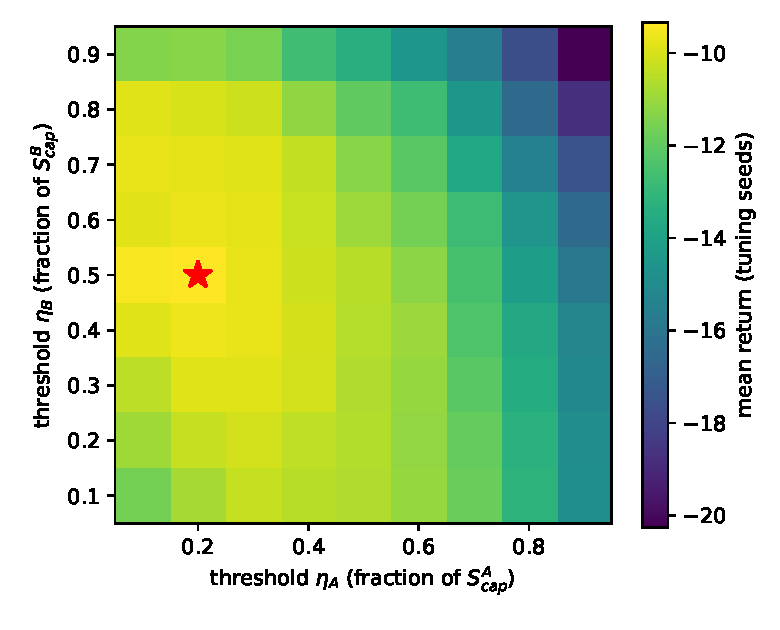
\includegraphics[width=0.55\textwidth]{figures/cascade_threshold_tuning.pdf}
\caption{Mean return of the cascade rule over its two thresholds (tuning
seasons). The star marks the tuned rule.}
\label{fig:cascade_tuning}
\end{figure}

\subsection{Training}
PPO uses the same networks and hyperparameters as in Section~\ref{sec:ppo},
with 16 inputs and two action dimensions, for about $10^6$ environment
steps with 16 workers (about 670 steps/s).
Training took about 28 minutes, about $10^6$ simulated days or 11{,}000
seasons, each day a full OHQ run of the two-reservoir model.
Figure~\ref{fig:cascade_learning} shows the return rising from about $-44$
(an untrained, essentially random policy) to about $-11$ after 160{,}000
steps, and to the $-4$ to $-9$ range after 500{,}000 steps. The curve stays
jagged because it averages only the last 20 training seasons, and those
seasons differ in storminess (and are run with exploration noise on). The
exploration spread $\sigma$ falls steadily from 0.59 to 0.18. The agent
becomes more confident but still explores, so more training might still
help a little.


\begin{figure}[h]
\centering
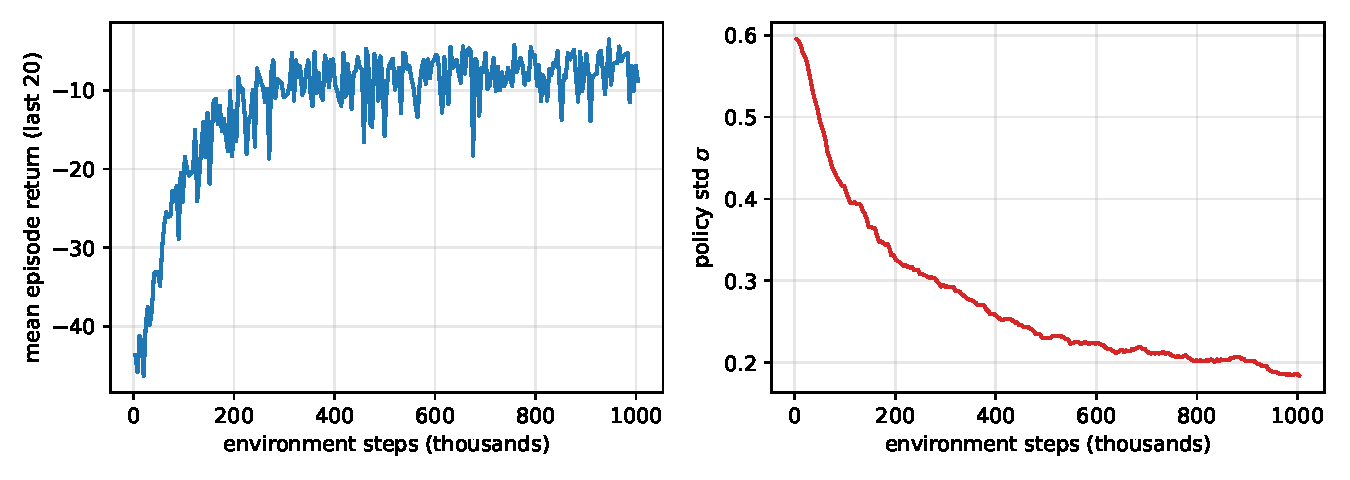
\includegraphics[width=0.95\textwidth]{figures/cascade_learning_curve.pdf}
\caption{Cascade training: mean return of the last 20 episodes (left) and
the mean policy standard deviation (right).}
\label{fig:cascade_learning}
\end{figure}

\subsection{Results}
All policies are evaluated on the same 30 held-out seasons (seeds
$10{,}000$--$10{,}029$). The tuned thresholds are
$\eta_A=0.2$, $\eta_B=0.5$.

\begin{table}[h]
\centering
\small
\begin{tabular}{lrrrrrrr}
\toprule
Policy & Return & Supply & Flood & Spill & Terminal & Deficit [\%] & Flood days \\
\midrule
Supply only & $-38.59\pm38.93$ & -1.12 & -14.23 & -22.74 & -0.50 & 3.1 & 9.4 \\
Rule (0.6, 0.5) & $-15.94\pm22.12$ & -1.18 & -7.41 & -6.64 & -0.71 & 2.8 & 8.2 \\
Tuned rule (0.2, 0.5) & $-14.07\pm19.26$ & -2.19 & -6.30 & -4.48 & -1.10 & 5.1 & 11.4 \\
PPO & $-12.27\pm17.30$ & -1.78 & -6.01 & -3.45 & -1.03 & 5.3 & 8.5 \\
\bottomrule
\end{tabular}

\caption{Cascade: mean over 30 test seasons, with columns as in
Table~\ref{tab:results}.}
\label{tab:cascade_results}
\end{table}

\begin{table}[h]
\centering
\begin{tabular}{lrrr}
\toprule
baseline & mean(PPO $-$ baseline) & std.\ error & PPO better in \\
\midrule
Supply only & $+26.32$ & 5.47 & 21/30 \\
Rule (0.6, 0.5) & $+3.67$ & 1.34 & 18/30 \\
Tuned rule (0.2, 0.5) & $+1.79$ & 0.67 & 22/30 \\
\bottomrule
\end{tabular}

\caption{Cascade: paired differences in season return, PPO minus
baseline.}
\label{tab:cascade_paired}
\end{table}

\paragraph{Headline.} In the cascade, PPO beats every baseline, including
the rule with tuned thresholds. Against the tuned rule, the season-by-season
difference is $+1.79\pm0.67$: about 2.7 standard errors, with PPO better in
22 of the 30 test seasons (Table~\ref{tab:cascade_paired}). In the
single-reservoir problem the same comparison was a statistical tie. The
extra difficulty of coordinating two reservoirs around an uncontrolled
tributary is what lets the learned policy pull ahead. The size of the gain
over the tuned rule is modest (about 13\% of its penalty), but it is
consistent.

\paragraph{Where the gain comes from.} Table~\ref{tab:cascade_results}
splits the return into its parts. Compared with the tuned rule, PPO
spills 23\% less water (13{,}800 versus 17{,}900~m$^3$ per season), floods
the river on fewer days (8.5 versus 11.4), and has a slightly smaller
supply penalty with the same total shortfall ($\approx5\%$ of demand). The
three trajectory figures show the mechanisms:
\begin{itemize}
\item \textbf{Hedging in droughts (Figure~\ref{fig:cascade_traj_med}).}
In this median season a long dry spell empties both reservoirs under every
policy. The rules deliver the full demand until the water runs out and
then deliver almost nothing for about 20 days. PPO starts delivering
somewhat less than demand around day 15, \emph{before} the reservoirs are
empty, and stretches its storage further. Because the supply penalty is
\emph{squared}, many small shortfalls cost less than a few large ones:
spreading a 1{,}000~m$^3$/d deficit over twice as many days at half the
size halves its penalty. This is the classic \emph{hedging rule} of
reservoir operation theory. The agent was never told about it; it
discovered it from the shape of the reward.
\item \textbf{Anticipating storms (Figure~\ref{fig:cascade_traj_best}).}
In this storm-rich season PPO raises releases ahead of forecast storms, up
to and slightly above $\Qsafe$, and keeps more room in B, so the storms
around days 40--47 cause far less spill than under the rules.
\item \textbf{Where it loses (Figure~\ref{fig:cascade_traj_worst}).} In
the season where PPO does worst relative to the tuned rule, a cluster of
storms arrives at the very end of the season. The tuned rule happened to
be holding A very low (its 20\% threshold) and absorbed more of it. PPO,
which also weighs the end-of-season storage term, was fuller and spilled
more. A learned policy is better \emph{on average}, not in every season.
\end{itemize}

\paragraph{The rule baselines.} The threshold map
(Figure~\ref{fig:cascade_tuning}) shows the logic of the best rule: keep
the large upstream reservoir low ($\eta_A=0.2$) and the small downstream
one at half ($\eta_B=0.5$), so that A's slow, large storm volumes have room
while B buffers the fast local response. Even tuned, the rule cannot
\emph{change} these targets with the forecast or the season, and that
flexibility is what PPO adds. ``Supply only'', which never releases for
flood space, shows how much is at stake: it spills about 91{,}000~m$^3$ per
season and scores $-38.6$.

\paragraph{Lessons for applying RL.}
\begin{enumerate}\itemsep1pt
\item RL helps most where simple rules are structurally limited: several
interacting storages, uncontrolled inflows and forecasts. For one
reservoir, a well-tuned rule was as good.
\item The reward shapes the behavior. The hedging seen here follows from
the squared deficit penalty, and a linear penalty would not produce it.
\item Fair comparison requires tuned baselines, identical test seasons and
paired statistics. Against the untuned rule the gain would have looked
twice as large ($+3.7$).
\end{enumerate}


\begin{figure}[h]
\centering
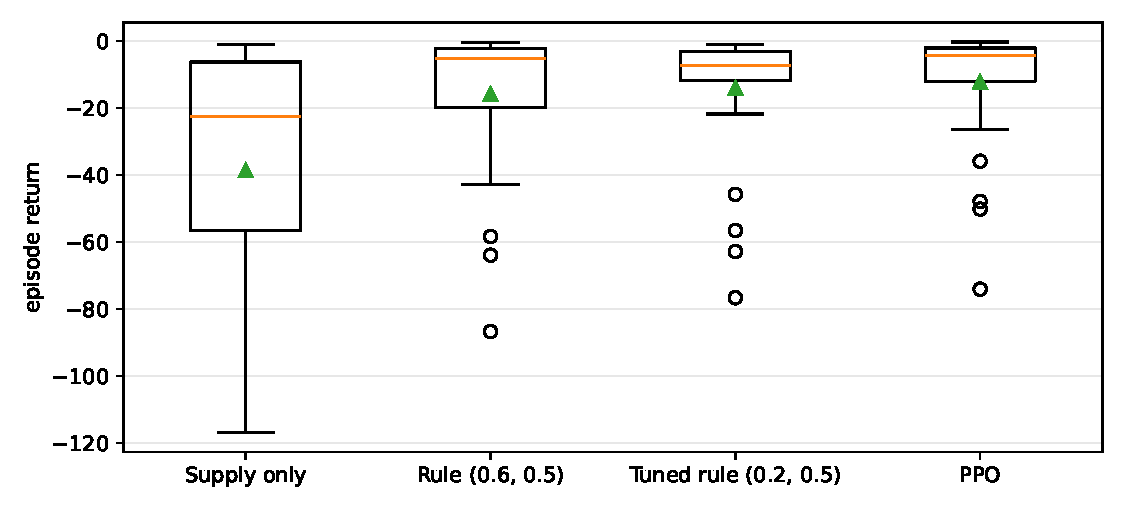
\includegraphics[width=0.7\textwidth]{figures/cascade_return_boxplot.pdf}
\caption{Cascade: distribution of test-season returns.}
\end{figure}

\begin{figure}[p]
\centering
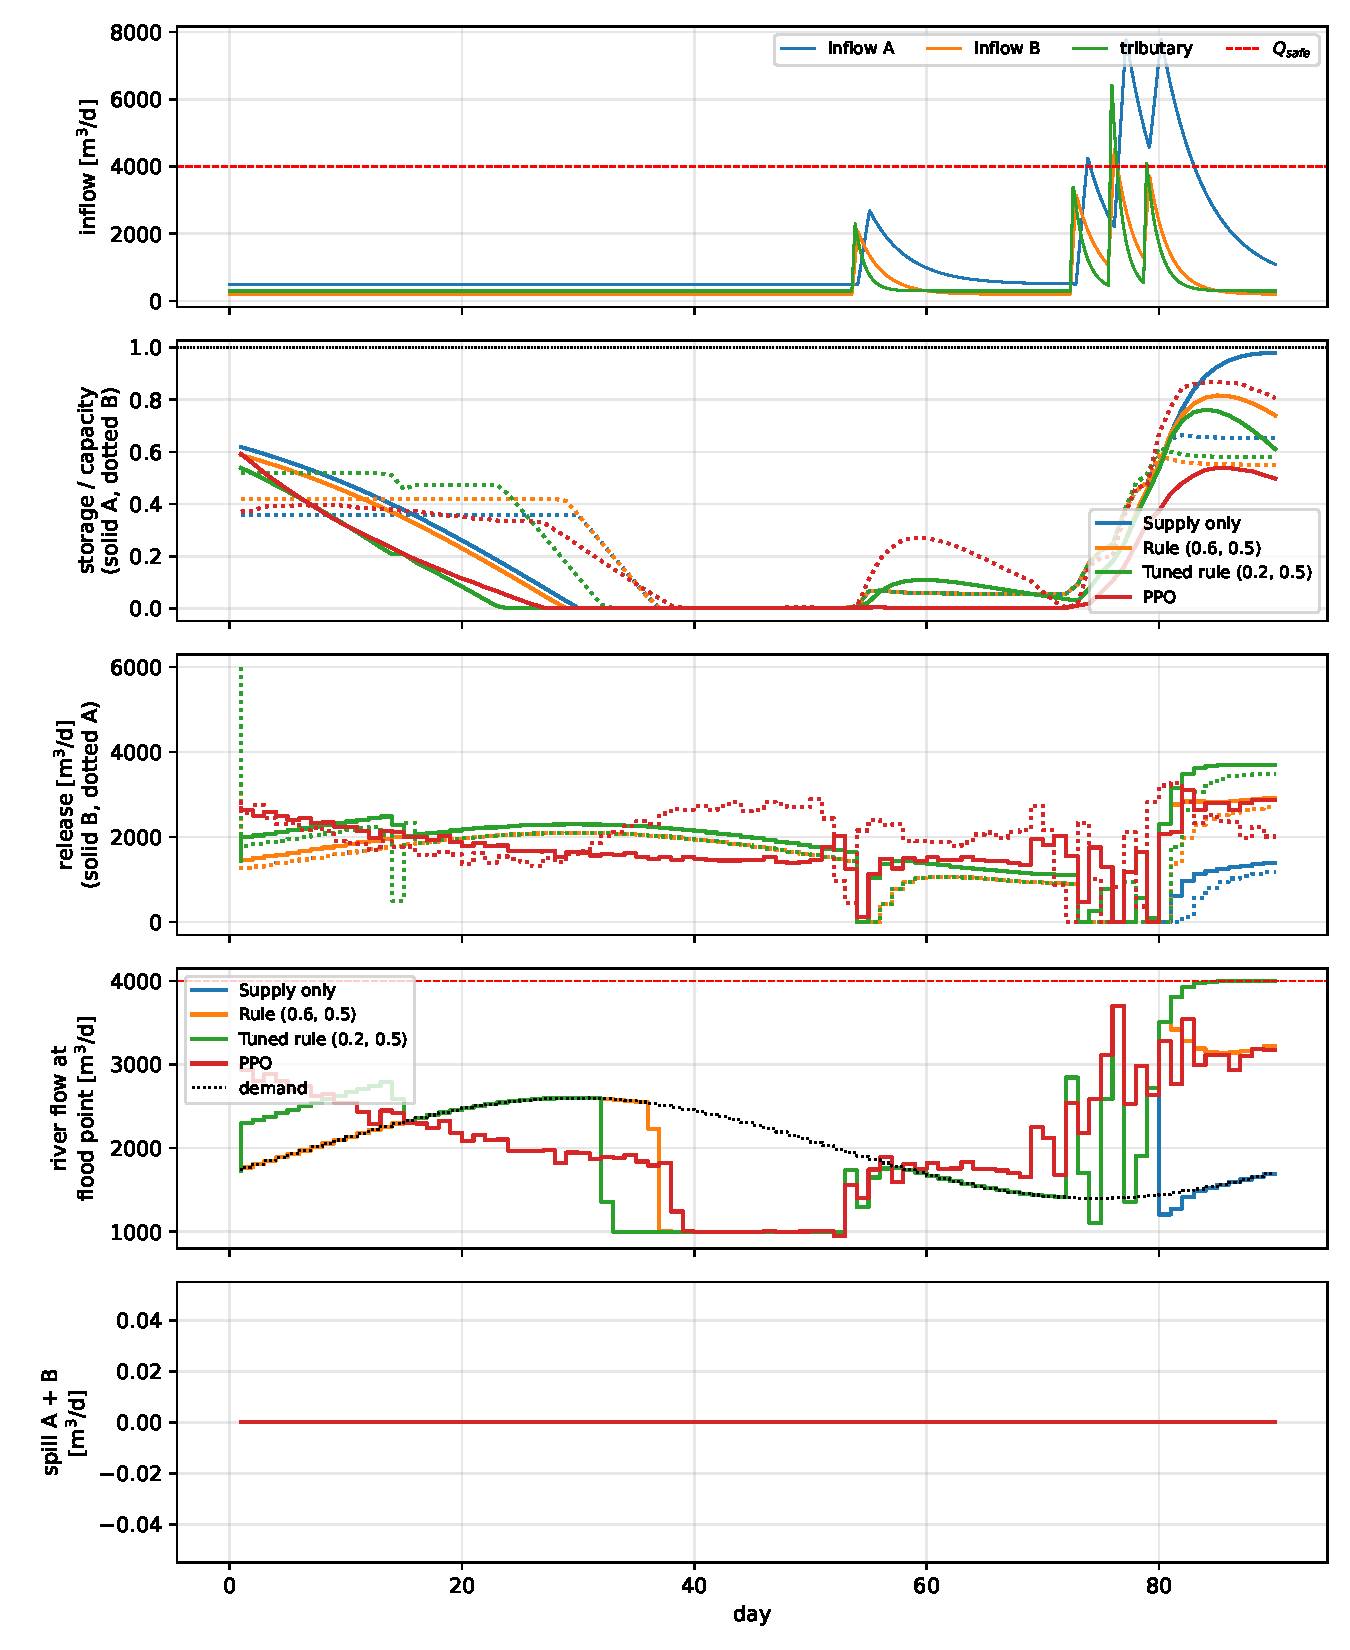
\includegraphics[width=0.92\textwidth]{figures/cascade_trajectory_median.pdf}
\caption{Cascade test season with the median PPO-vs-tuned-rule difference.
From top: the three inflows; storages (solid A, dotted B); releases (solid
B, dotted A); river flow at the flood point with demand (dotted) and
$\Qsafe$ (dashed); total spill.}
\label{fig:cascade_traj_med}
\end{figure}

\begin{figure}[p]
\centering
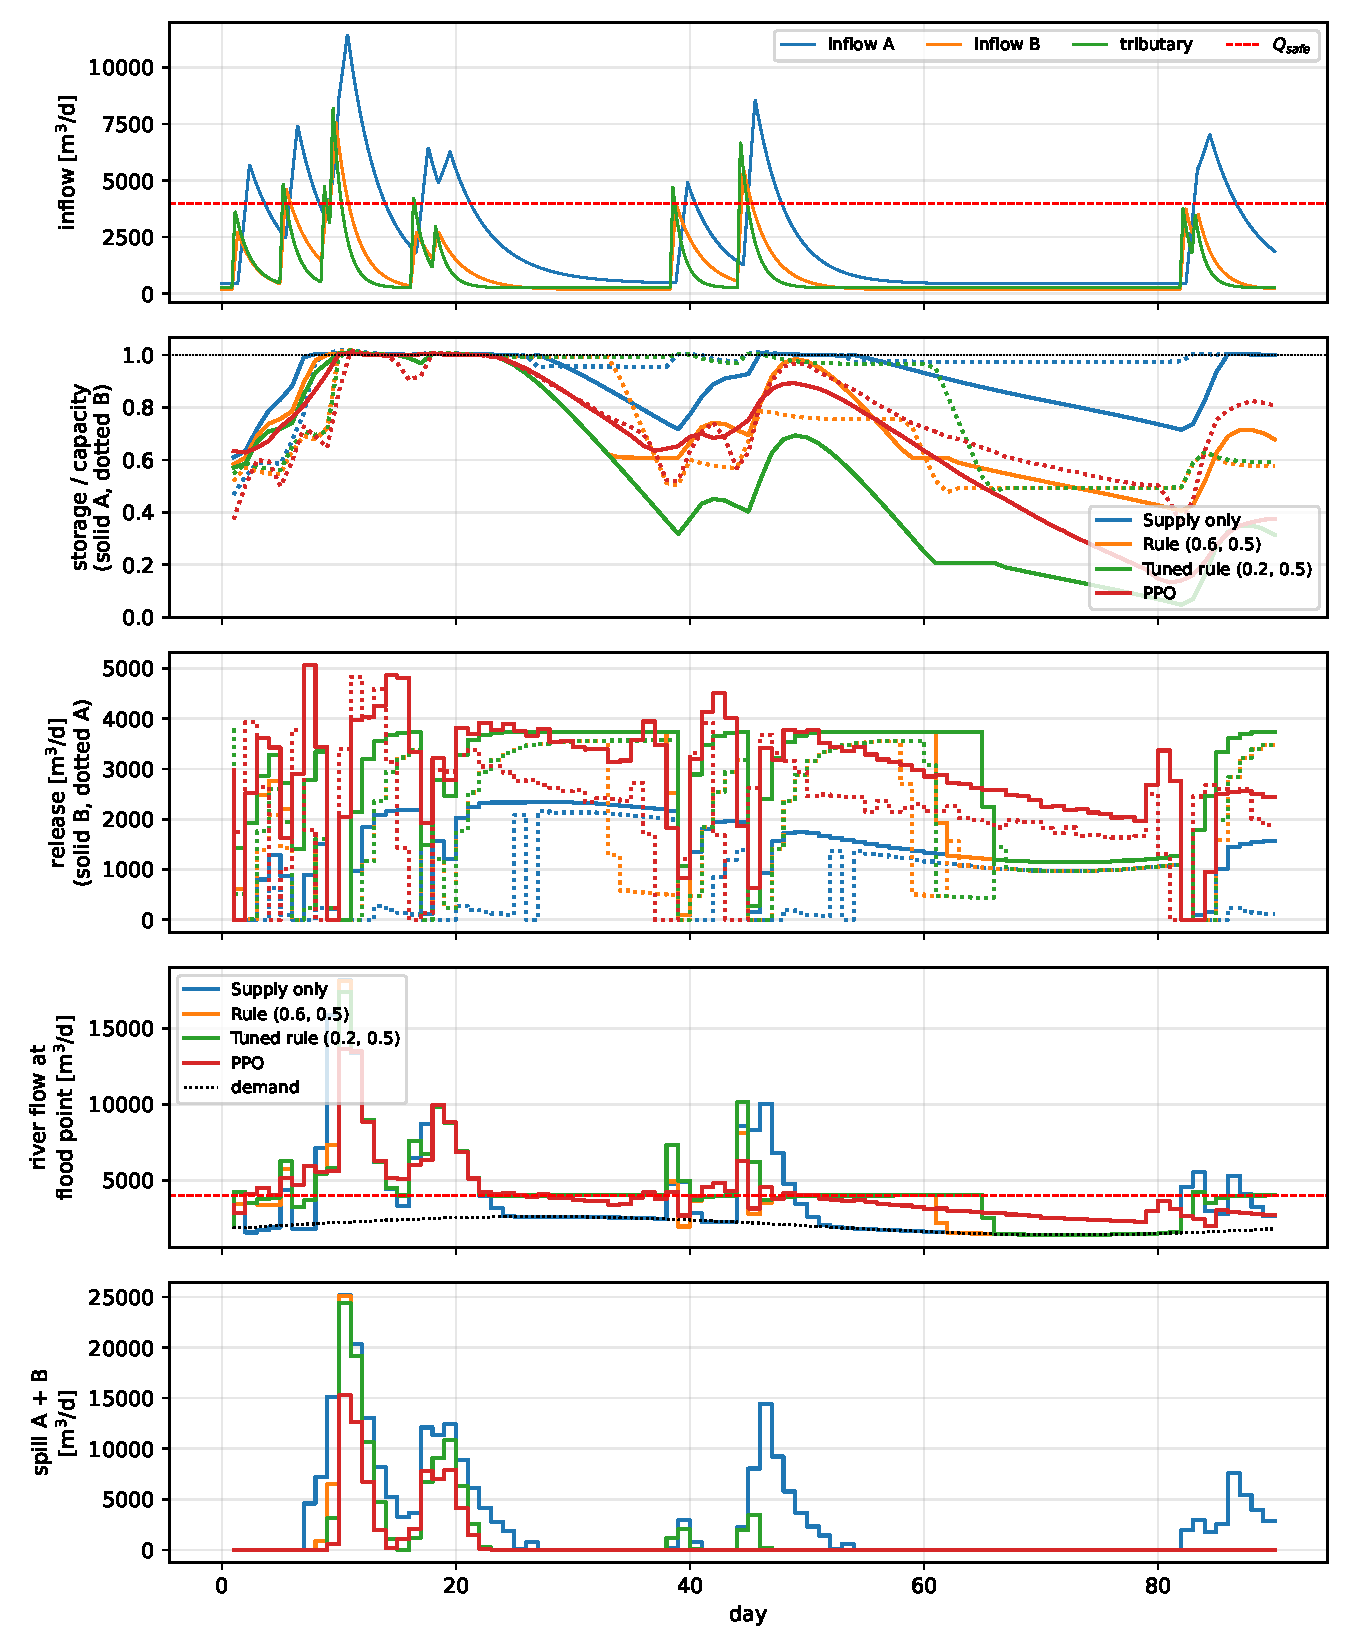
\includegraphics[width=0.92\textwidth]{figures/cascade_trajectory_best_gain.pdf}
\caption{Cascade test season with the largest PPO gain over the tuned rule.}
\label{fig:cascade_traj_best}
\end{figure}

\begin{figure}[p]
\centering
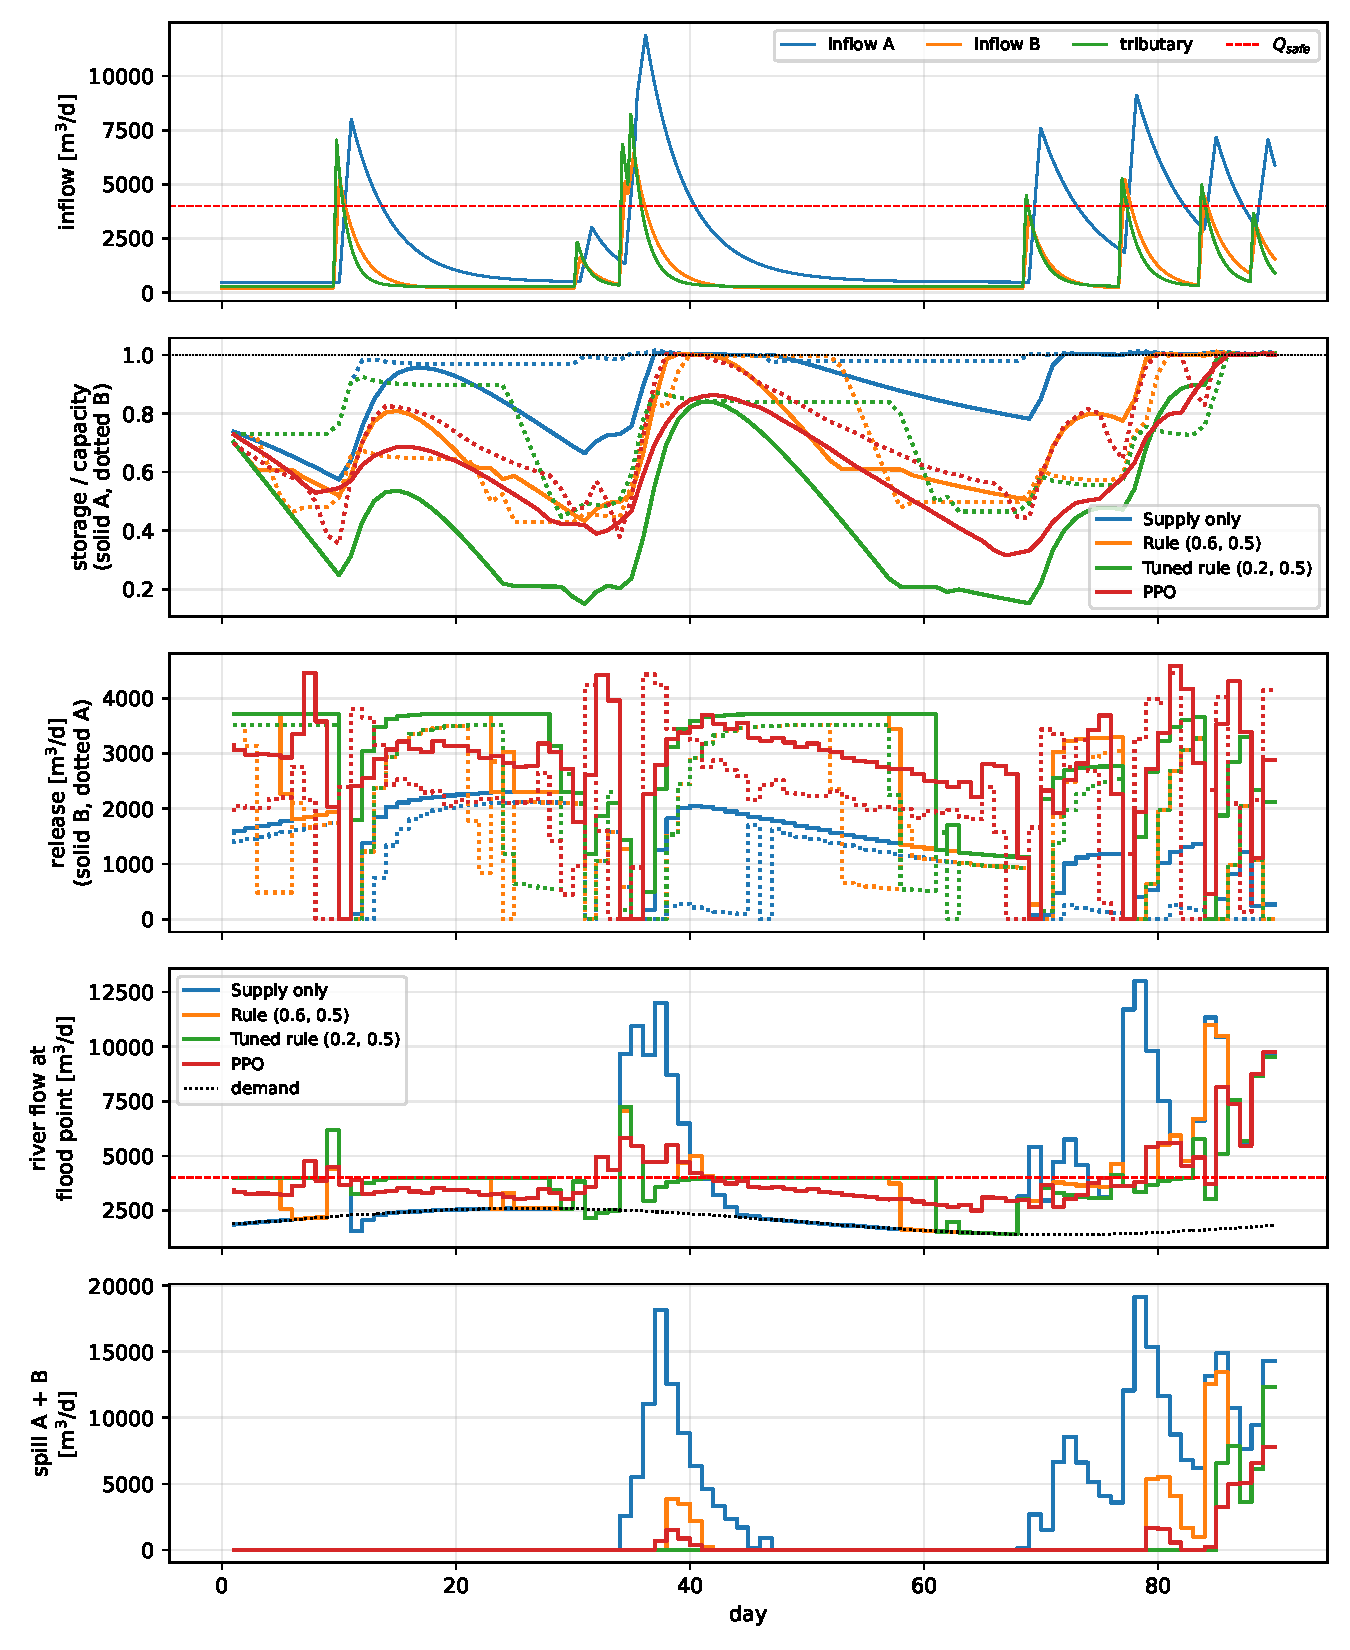
\includegraphics[width=0.92\textwidth]{figures/cascade_trajectory_worst.pdf}
\caption{Cascade test season where PPO does worst relative to the tuned rule.}
\label{fig:cascade_traj_worst}
\end{figure}


%=====================================================================
\section{A third problem -- real-time control of a stormwater pond}\label{sec:pond}
%=====================================================================

The third problem changes the time scale from days to hours and adds a
water-quality objective. A stormwater pond collects runoff from an
impervious catchment and releases it through a valve that can be opened or
closed every hour. The pond has two jobs that pull in opposite directions:
\begin{itemize}\itemsep1pt
\item \textbf{Peak-flow control:} keep the outflow downstream low. We
measure this with $Q_p$, the outflow exceeded only a fraction $p$ of the
time (the ``exceedance'' objective of OHQ, as in the St.~Francis
real-time-control study).
\item \textbf{Treatment:} hold water long enough for pollutants to settle
and degrade. We measure this with the \emph{young-water fraction} of the
outflow from OHQ's Laplace age tracer.
\end{itemize}
Holding water (valve nearly closed) makes it older, which is good for
treatment. But the pond is then full when the next storm arrives and it
overflows, which is bad for $Q_p$. Releasing keeps room but passes young,
untreated water. A good operator holds water in dry weather and makes room
before storms, which is a natural job for a forecast-aware learned policy.

\subsection{System and data}
\begin{figure}[h]
\centering
\resizebox{\textwidth}{!}{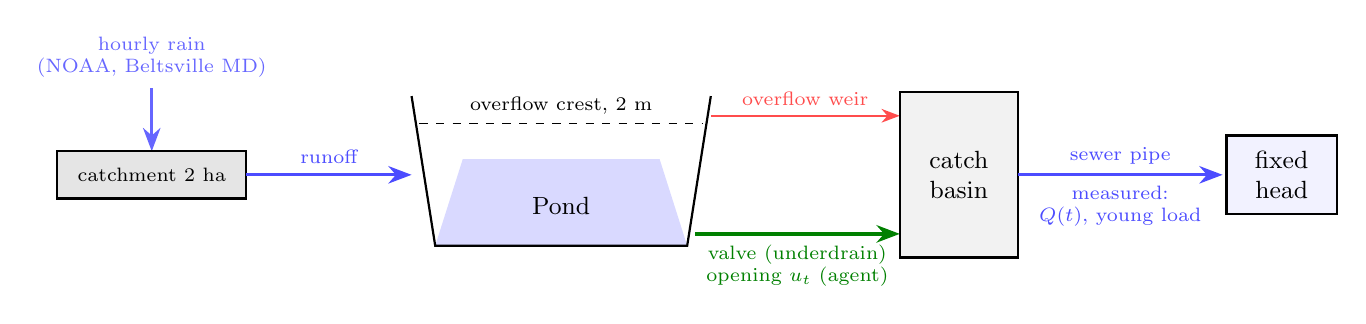
\begin{tikzpicture}[>=Stealth, font=\small]
  \draw[->, very thick, blue!60] (-4.2,1.6) node[above, font=\scriptsize, align=center]{hourly rain\\(NOAA, Beltsville MD)} -- (-4.2,0.8);
  \draw[thick, fill=gray!20] (-5.4,0.2) rectangle (-3.0,0.8);
  \node[font=\scriptsize] at (-4.2,0.5) {catchment 2 ha};
  \draw[->, very thick, blue!70] (-3.0,0.5) -- node[above, font=\scriptsize]{runoff} (-0.9,0.5);
  \fill[blue!15] (-0.6,-0.4) -- (-0.25,0.7) -- (2.25,0.7) -- (2.6,-0.4) -- cycle;
  \draw[thick] (-0.9,1.5) -- (-0.6,-0.4) -- (2.6,-0.4) -- (2.9,1.5);
  \draw[dashed] (-0.8,1.15) -- (2.8,1.15);
  \node[font=\scriptsize, above] at (1.0,1.15) {overflow crest, 2 m};
  \node at (1.0,0.1) {Pond};
  \draw[->, very thick, green!50!black] (2.7,-0.25) -- node[below, font=\scriptsize, align=center]{valve (underdrain)\\opening $u_t$ (agent)} (5.3,-0.25);
  \draw[->, thick, red!70] (2.9,1.25) -- node[above, font=\scriptsize]{overflow weir} (5.3,1.25);
  \node[draw, thick, fill=gray!10, minimum width=1.5cm, minimum height=2.1cm, align=center, font=\small] (cb) at (6.05,0.5) {catch\\basin};
  \draw[->, very thick, blue!70] (6.8,0.5) -- node[above, font=\scriptsize]{sewer pipe} node[below, font=\scriptsize, align=center]{measured:\\$Q(t)$, young load} (9.4,0.5);
  \node[draw, thick, fill=blue!5, minimum width=1.4cm, minimum height=1.0cm, align=center, font=\small] at (10.15,0.5) {fixed\\head};
\end{tikzpicture}}
\caption{The stormwater pond. Both the valve (underdrain) and the overflow
discharge into a catch basin, which drains to the receiving water (a fixed
head) through a sewer pipe. Flow and young-water load are measured on that
pipe.}
\label{fig:pond_schematic}
\end{figure}

\paragraph{Rainfall.} The pond is driven by observed rainfall from NOAA's
Hourly Precipitation Data network (HPD v2, NOAA NCEI): station USC00180700,
Beltsville, Maryland, which lies between Baltimore and Washington DC. The
record runs from 1948 to 2026 at hourly resolution. Values are converted from
hundredths of an inch to meters, and flagged or missing hours are kept as
gaps (\code{prepare\_rain.py}). Annual totals of 1{,}000--1{,}200~mm, and a
record 1{,}804~mm in 2018, match the regional climatology. Each episode is a
\textbf{three-year} window (26{,}280 hours), as in the St.~Francis study.
A short window lets a controller exploit end effects (see ``Closing
loopholes'' below), and $Q_p$ at a small $p$ needs a long record. No
three-year window is entirely complete, so windows may have at most 1\%
missing hours, which are taken as dry. Training windows start anywhere in
1980--2019 where this holds (in practice 1996--2017 starts, about 12
distinct years of weather). The test windows are the two disjoint periods
2020--2022 and 2023--2025, which the agent never sees. Because two windows
give weak statistics, the comparison is also made year by year (six test
years).

\paragraph{Catch basin.} Following the St.~Francis model, the valve and the
overflow weir both discharge into a \code{Catch basin} block (4~m$^2$,
\code{Sewer\_system.json}). It drains through a \code{Sewer\_pipe} (0.3~m
diameter, Manning $n=0.01$, 10\% slope; capacity about 34{,}000~m$^3$/d) to
a fixed head. Measuring at the pipe means that overflow water is counted
with the tracer concentration OHQ actually carries through the system.

\paragraph{Catchment and pond.} Runoff is the rain on a 2-ha impervious
catchment with runoff coefficient 0.9, entering the pond as a
piecewise-constant hourly inflow. The pond is OHQ's \code{Pond} block
(\code{Pond\_Plugin.json}), whose storage--depth relation is approximately
$S=\alpha h^\beta$, with $\alpha=250$, $\beta=2$. The overflow crest at
$h=2$~m corresponds to 1{,}000~m$^3$, about 55~mm of runoff from the
catchment. An overflow
weir (\code{wier}, $Q=440{,}000\,(h-2)^{1.5}$~m$^3$/d) discharges anything
above the crest.

\paragraph{The valve.} The valve is a new OHQ link type,
\code{controlled\_orifice} (added to \path{resources/Pond_Plugin.json}
during this work): the orifice law with the valve opening $u\in[0,1]$ as a
property,
\[
Q_{valve}=86400\,C_d\,u\,A_{max}\sqrt{2g}\;\frac{h}{\sqrt{h+\varepsilon}},
\qquad C_d=0.6,\ A_{max}=0.03~\text{m}^2,\ \varepsilon=1~\text{mm}.
\]
The factor $h/\sqrt{h+\varepsilon}$ equals $\sqrt h$ for any real head but
becomes linear near an empty pond. With the plain $\sqrt h$ law, whose
slope is infinite at $h=0$, the implicit solver failed whenever an open
valve drained the pond within an hour. The St.~Francis valve devices use
the same regularization. While checking this link against a hand
calculation, we found that OHQ currently evaluates a function of a
\emph{pure constant} as the constant itself: $\sqrt{19.6}$ written as
\code{\_sqr(19.6)} evaluated to 19.6, which made the valve 4.4$\times$ too
large. The link type therefore writes $\sqrt{2g}=4.427$ as a number, so that it
also works with library builds that predate the fix of that bug (since
committed to OHQ). Here $h$ is the head difference between the pond and the
catch basin.

\subsection{Measuring water age with the Laplace tracer}
OHQ's \code{AgeTracker\_laplace} constituent, set up exactly as in the
St.~Francis residence-time study (\code{add\_age.py}), carries a tracer at
concentration 1 in every inflow. The tracer decays at a first-order rate
$\lambda$ wherever it is. A parcel of water that has spent time $\tau$ in
the system therefore carries concentration $e^{-\lambda\tau}$. If the water
in the pond (or leaving it) is a mixture of parcels with age density
$p(\tau)$, its concentration is
\[
C=\int_0^\infty p(\tau)\,e^{-\lambda\tau}\,d\tau=\mathcal L\{p\}(\lambda),
\]
the Laplace transform of the age distribution evaluated at $s=\lambda$:
hence the name. With $\lambda=1$~d$^{-1}$, water younger than a few hours
counts almost fully ($e^{-\lambda\tau}\approx1$) and water older than a few
days hardly at all. So $C$ acts as a smooth ``fraction of young water'' with
a time scale of about one day. The \textbf{young-water fraction} of the
outflow over an episode is the exported tracer load divided by the outflow
volume:
\[
F_y=\frac{\int Q(t)\,C(t)\,dt}{\int Q(t)\,dt}.
\]

\subsection{OHQ model and checks}
The Python binding cannot create constituents or reactions, so each hour's
model is written as a small \code{.ohq} script and loaded with
\code{create\_from\_script}. The script holds the templates, the tracer and
its decay reaction, the pond (with the current storage and tracer
concentration as initial conditions), the valve with this hour's opening,
the weir and the outlet. It is solved with twelve 5-minute steps, again
single-threaded. The pipe's hourly volume and young-water load are taken
from the catch basin's balance: inflow from the pond (valve and weir fluxes
at the end-of-step pond state, the valve seeing the basin's water level)
minus the change in the basin's water and tracer content, minus tracer
decay in the basin. This is exact by construction, whereas integrating
OHQ's interpolated rate outputs left a 3\% balance error. The pipe-flow
samples from OHQ's output give the 5-minute flows used for $Q_p$. Checks:
\begin{itemize}\itemsep1pt
\item \textbf{Valve law:} the outflow implied by OHQ's storage drop over a
step matches the formula above, evaluated at the end-of-step depth
(backward Euler), to within 0.1\%.
\item \textbf{Tracer:} closed valve, $S_0=1{,}900$~m$^3$, $C_0=0.3$, inflow
2{,}000~m$^3$/d for one hour. A hand mass balance (tracer inflow $+83.3$,
decay $\lambda M\,\Delta t\approx-23.8$) gives $C\approx0.317$; OHQ gives
0.3168.
\item \textbf{Water balance} over 800-hour test runs closes to within
0.01~m$^3$ out of 1{,}400--3{,}100~m$^3$ of inflow.
\end{itemize}
\paragraph{Making it fast enough.} A typical hourly step costs 20--50~ms:
about 23~ms to parse the script and templates, plus the solve. Three
problems had to be fixed first:
\begin{enumerate}\itemsep1pt
\item \textbf{Inflow file.} OHQ re-reads the inflow time series at every
build. A whole-episode file (52{,}000 points for three years) made each
step take seconds, so each step now gets a two-point file for its own hour.
\item \textbf{Round-off states.} When the pond or catch basin empties,
storages of $10^{-7}$--$10^{-11}$~m$^3$ and decayed tracer concentrations
of $10^{-150}$ made OHQ's Newton iterations crawl, at 1--2~s per hour.
Values below 0.1~m$^3$ (pond) and 0.01~m$^3$ (basin) are therefore set to
exactly zero between steps.
\item \textbf{Lockstep rollouts.} Even then about 0.6\% of hours take
around a second. With 16 simulators advanced in lockstep, every step
waited for the slowest, and throughput collapsed to about 20 steps/s. The
trainer now lets each worker collect its rollout independently
(Section~\ref{sec:ppo}).
\end{enumerate}
At 20--50~ms per step, a three-year episode costs about 15--20 minutes of
CPU, the clearest case so far for a compiled (codegen) backend.

\subsection{Objectives, reward and the exceedance problem}
\paragraph{Evaluation metrics.} For each test window we compute, from the
outflow at every 5-minute solver step:
\begin{itemize}\itemsep1pt
\item $Q_p$ with $p=0.001$: the flow exceeded 0.1\% of the time (about 43
minutes per month), the value used in the St.~Francis study;
\item the young-water fraction $F_y$;
\item a scalar objective used to tune baselines and rank policies, with
each metric normalized by the \emph{passive} pond (valve fully open) under
the same rain:
\[
J=\frac{Q_p}{Q_p^{\,passive}}+\frac{F_y}{F_y^{\,passive}} .
\]
Lower is better. The passive pond scores exactly 2, and halving either
metric relative to doing nothing is worth the same. The normalization is
done per test window and per test year. For the tuning grid it uses the
passive pond's averages over the two tuning windows. Because any weighting
is a judgment call, we also show the full trade-off between $Q_p$ and
$F_y$.
\end{itemize}

\paragraph{Closing loopholes.} Earlier versions of this problem show how
readily an optimizer exploits gaps in an objective:
\begin{itemize}\itemsep1pt
\item With a pond twice as large (2{,}000~m$^3$) and 30-day episodes, the
best tuned rule kept the valve shut all month. A month's runoff fit in the
pond, so almost nothing left and $Q_p$ was near zero, and every window
ended with a full pond, a cost the window never saw. A realistically sized
pond (1{,}000~m$^3$) and three-year episodes remove this.
\item Water still in the pond or catch basin at the end of an episode is
counted as exported at its current tracer concentration, so holding water
to the end cannot hide young water.
\item With 30-day episodes, PPO learned to keep the pond near the crest and
let it overflow in short bursts. In the first model the overflow went
straight to the outlet and the age tracer treated it as old pond water.
Routing both the valve and the overflow through the catch basin, and
measuring there, makes OHQ carry the overflow's age consistently.
\end{itemize}
Following the design intent, there is no explicit penalty on overflow and
no minimum-storage rule. Overflow matters only through its effect on the
exceedance flow and on the young-water fraction, and the agent is free to
use it whenever that helps.

\paragraph{Choosing $p$.} We first used $p=0.01$. Over a 30-day window that
is about 7 hours, and a short overflow lasting less than that falls entirely
inside the ignored 1\%. A rule that kept the valve shut and let the pond
overflow scored a $Q_p$ of only 264~m$^3$/d despite overflow peaks of
8{,}800~m$^3$/d. With $p=0.001$, $Q_p$ reflects such peaks, and the training
surrogate (which penalizes every high flow) and the evaluation metric agree.

\paragraph{Why not use $Q_p$ as the reward directly?} RL maximizes a
\emph{sum} of per-step rewards (Section~\ref{sec:primer_math}). A quantile
is not a sum: whether a particular hour's flow matters depends on all other
hours of the episode. Its only exact form would be a single reward at the
very end of the 720-hour episode, which gives the agent almost no signal
about which hours mattered. We therefore train on a smooth
\emph{surrogate} that is additive, and evaluate on the exact $Q_p$:
\[
r_t=-w_q\,\frac{1}{\Delta t}\sum_{n}\Big(\frac{\max(0,\,Q_n-Q_{ref})}{Q_{ref}}\Big)^2\delta t
\;-\;w_y\,\frac{\sum_n Q_n C_n\,\delta t}{V_{ref}},
\]
summed over the solver steps $n$ of hour $t$. The first term penalizes
flows above $Q_{ref}$, and penalizes large ones much more because of the
square, which pushes down the upper tail of the flow distribution, where
$Q_p$ lives. The second term is the exported young-water load, which is
additive, so it represents $F_y$ exactly up to the (nearly policy-independent)
total outflow volume. Here $w_q=1$, $w_y=5$ and $V_{ref}=1{,}000$~m$^3$. The
weights roughly mirror $J$: with $Q_p^{\,passive}\approx5{,}000$~m$^3$/d and
$F_y^{\,passive}\approx1$, $J\propto Q_p/1{,}000+5F_y$.

\paragraph{Observation and action.} The agent observes 9 numbers: pond
depth, pond tracer concentration $C$, current inflow, noisy rain forecasts
for the next 1, 3, 6, 12 and 24 hours (multiplicative log-normal error
growing with lead time), and the fraction of the window left. It sets the
valve opening once per hour. The network's action $a_t\in[-1,1]$ is mapped
to the opening as $u_t=((a_t+1)/2)^2$. With the linear mapping used at
first, the useful openings of 0--10\% occupied only the bottom 5\% of the
action range; with the square they occupy about a third of it.

\subsection{Baselines}
\begin{itemize}\itemsep1pt
\item \textbf{Open valve} ($u=1$): a conventional dry pond with a fixed
orifice.
\item \textbf{Fixed opening} $u$: a throttled orifice; $u$ tuned over $\{0.03,0.05,0.1,0.2,1\}$.
\item \textbf{Forecast rule}, in the spirit of the St.~Francis
forecast-informed control: hold at a small opening $u_{hold}$ so that water
ages; when the 24-hour rain forecast exceeds a threshold, pre-release at
$u_{pre}$; open fully if the depth exceeds 1.8~m. The three parameters are
tuned by grid search over 24 combinations ($u_{hold}\in\{0,0.02\}$, $u_{pre}\in\{0.05,0.1,0.2,0.4\}$, threshold $\in\{10,15,30\}$~mm), centred on the best settings found with 30-day windows.
\end{itemize}
Both rule families are tuned on two three-year training-period windows
(starting 1996 and 2009); the results are fixed opening $u=0.02$; forecast rule $u_{hold}=0$, $u_{pre}=0.1$, threshold 15~mm.

\begin{figure}[h]
\centering
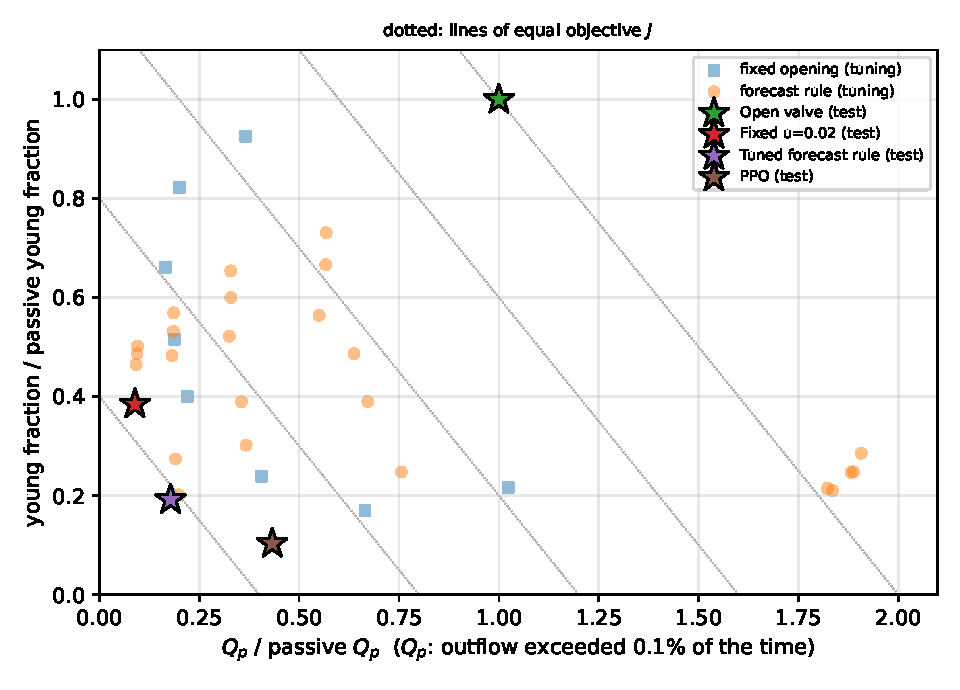
\includegraphics[width=0.7\textwidth]{figures/pond_tradeoff.pdf}
\caption{Trade-off between peak-flow control ($Q_p$) and treatment (young
fraction). Small symbols: every baseline setting tried during tuning
(training windows). Stars: the four compared policies on the test windows.
Dotted lines connect points with equal objective $J$.}
\label{fig:pond_tradeoff}
\end{figure}

\subsection{Training}
The first attempt trained PPO from scratch with a linear action mapping and
raw rewards. It converged to a poor policy that opened the valve only when
the pond was already empty, kept the pond at the crest, and scored a
normalized $J$ of 1.13--1.23 on the test windows, barely better than the
passive pond's 2. The run evaluated in Tables~\ref{tab:pond_results} and~\ref{tab:pond_paired}
uses the three remedies described in
Section~\ref{sec:ppo}: the square action mapping, reward normalization, and
a warm start by behavior cloning of the tuned forecast rule. The cloned
actor reproduced the rule's 48{,}000 decisions to within 0.008 on the action
scale. PPO then trained for 1.5 million hourly steps, about 2.5 hours on a
machine shared with other jobs. Its first rollouts already scored at the
rule's level (about $-0.005$ per hour, versus $-0.10$ from scratch). The
raw reward per hour kept improving to about $-0.0004$ by the end, and the
exploration spread fell from 0.30 to 0.13. A second warm-started run without reward clipping, with snapshot selection by $J$, is
described at the end of the results.


\begin{figure}[h]
\centering
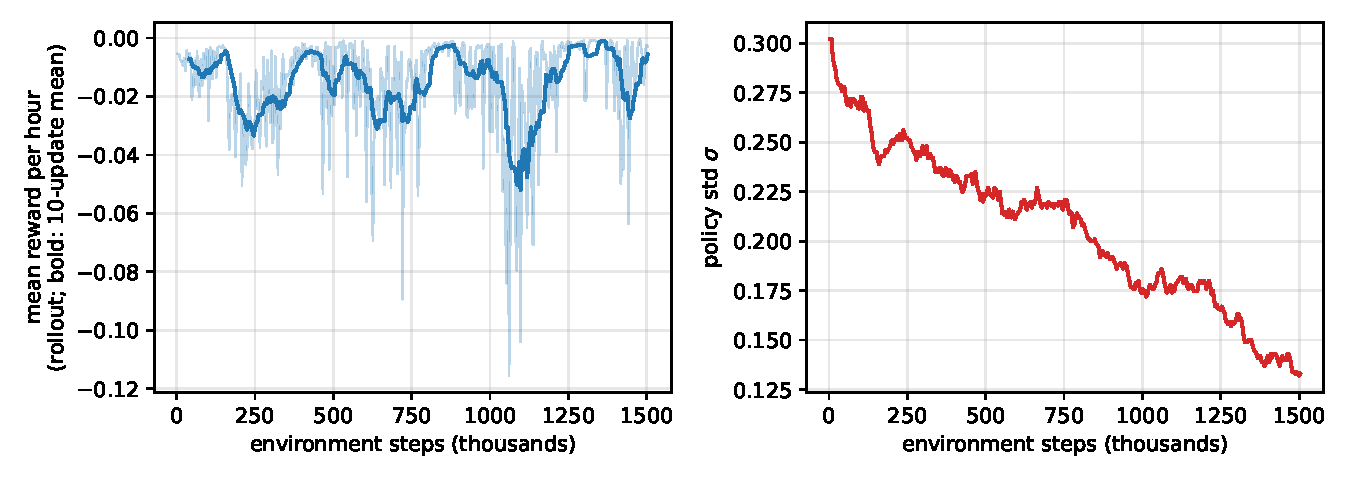
\includegraphics[width=0.95\textwidth]{figures/pond_learning_curve.pdf}
\caption{Pond training: mean return of the last 20 episodes (left), policy
standard deviation (right).}
\label{fig:pond_learning}
\end{figure}

\subsection{Results}
\begin{table}[h]
\centering
\small
\begin{tabular}{lrrrrrr}
\toprule
Policy & window & $J$ & $Q_p$ [m$^3$/d] & young fraction & peak [m$^3$/d] & overflow [m$^3$] \\
\midrule
Open valve & 2020--22 & 2.00 & 5182 & 0.993 & 8391 & 0 \\
 & 2023--25 & 2.00 & 4971 & 0.993 & 8558 & 0 \\
Fixed u=0.02 & 2020--22 & 0.50 & 697 & 0.361 & 11986 & 2349 \\
 & 2023--25 & 0.45 & 216 & 0.403 & 11525 & 1384 \\
Tuned forecast rule & 2020--22 & 0.37 & 912 & 0.197 & 12056 & 162 \\
 & 2023--25 & 0.36 & 896 & 0.183 & 11111 & 85 \\
PPO & 2020--22 & 0.59 & 2487 & 0.107 & 12309 & 11819 \\
 & 2023--25 & 0.48 & 1917 & 0.097 & 12195 & 6277 \\
\bottomrule
\end{tabular}

\caption{Pond: results for the two three-year test windows. $J$ is the
evaluation objective (lower is better).}
\label{tab:pond_results}
\end{table}

\begin{table}[h]
\centering
\small
\begin{tabular}{lrrrr}
\toprule
baseline & mean $\Delta J$ (per year) & std.\ error & PPO better in & mean $\Delta Q_p$ / $\Delta$young \\
\midrule
Open valve & $-1.494$ & 0.054 & 6/6 years & $-3031$ / $-0.892$ \\
Fixed u=0.02 & $+0.031$ & 0.050 & 2/6 years & $+1616$ / $-0.281$ \\
Tuned forecast rule & $-0.078$ & 0.216 & 2/6 years & $-12$ / $-0.088$ \\
\bottomrule
\end{tabular}

\caption{Pond: paired differences, PPO minus baseline, computed for each
of the six test years. Negative $\Delta J$ means PPO is better.}
\label{tab:pond_paired}
\end{table}

\paragraph{Headline.} Over the full three-year test windows, the tuned
forecast rule is the best policy ($J=0.375$ and 0.365, i.e.\ about 82\%
better than the passive pond). Next come the 2\% fixed opening (0.498,
0.450) and PPO (0.588, 0.483). Year by year, PPO and the rule are
statistically tied ($\Delta J=-0.08\pm0.22$, PPO better in 2 of 6 years).
The three-year metric, the St.~Francis definition, favors the rule because
PPO's overflows cluster in a few years and raise the three-year $Q_p$.
The warm start made a large difference: from scratch, PPO scored
$J\approx1.1$--1.2.

\paragraph{What PPO changed relative to the rule.} PPO started as an exact
copy of the rule and moved toward holding more water. Its outflow is the
oldest of all policies (young fraction 0.10--0.11, versus 0.18--0.20 for
the rule). But it ends both windows at the crest and overflows
6{,}000--12{,}000~m$^3$ per window (the rule: 85--162~m$^3$). Its $Q_p$ is
therefore 2--3 times the rule's. In terms of $J$, the gain in age does not
pay for the loss in peak-flow control.

\paragraph{Why: the training reward is not exactly $J$.} During training
PPO kept improving the reward it was given: the raw reward per hour
improved from $-0.028$ to $-0.0004$. That reward differs from $J$ in two
ways, and both undervalue overflow:
\begin{enumerate}\itemsep1pt
\item the peak term is a smooth surrogate of the exceedance quantile, not
the quantile itself;
\item reward normalization \emph{clips} rewards at $\pm10$ standard
deviations. That stabilized learning, but it also caps the penalty of
exactly the rare, extreme overflow hours that determine $Q_p$.
\end{enumerate}
So PPO optimized the stated reward well, but the stated reward traded
overflow for age at a different rate than $J$ does.

\paragraph{What would likely close the gap.}
\begin{itemize}\itemsep1pt
\item Normalize rewards without clipping (or with a much wider clip), so
the overflow penalty keeps its weight.
\item Select the policy by $J$: evaluate checkpoints during training on
held-out training-period windows and keep the best one, rather than the
last.
\item Keep the policy close to the rule unless it clearly improves on it,
e.g.\ by penalizing deviation from the cloned rule early in training.
\end{itemize}

\paragraph{Lessons.} Two lessons stand out. First, starting from an
engineering rule turned an RL failure into a policy competitive with a
carefully tuned rule. Second, when the true objective (a quantile over
three years) cannot be the reward, every simplification of it, including
the numerical stabilizations, becomes part of the objective the agent
actually optimizes. Whether the result is better must be judged on the
true objective, with tuned baselines, on data the agent has not seen.


\begin{figure}[h]
\centering
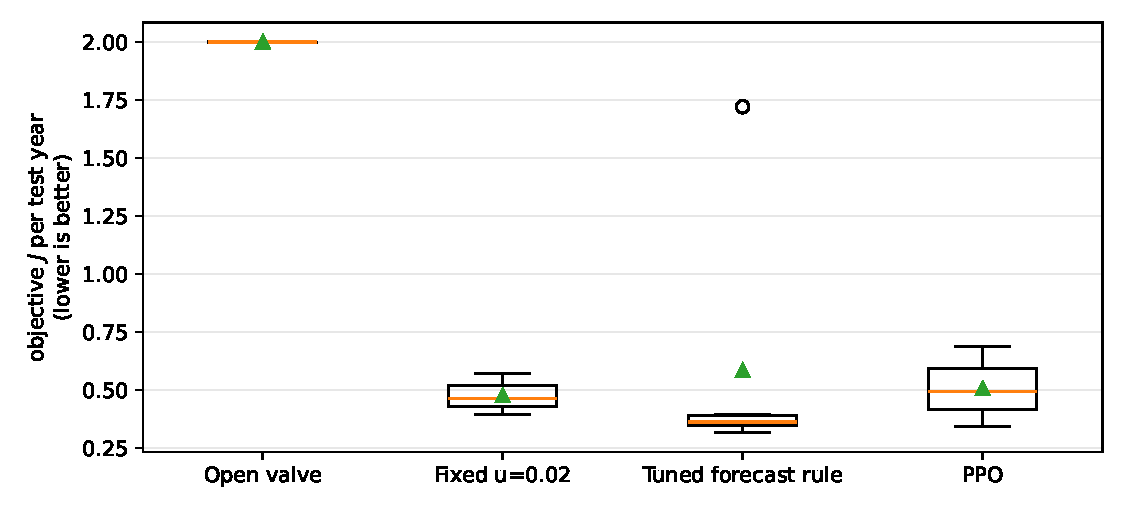
\includegraphics[width=0.7\textwidth]{figures/pond_J_boxplot.pdf}
\caption{Pond: distribution of the objective $J$ over the six test years.}
\end{figure}

\begin{figure}[p]
\centering
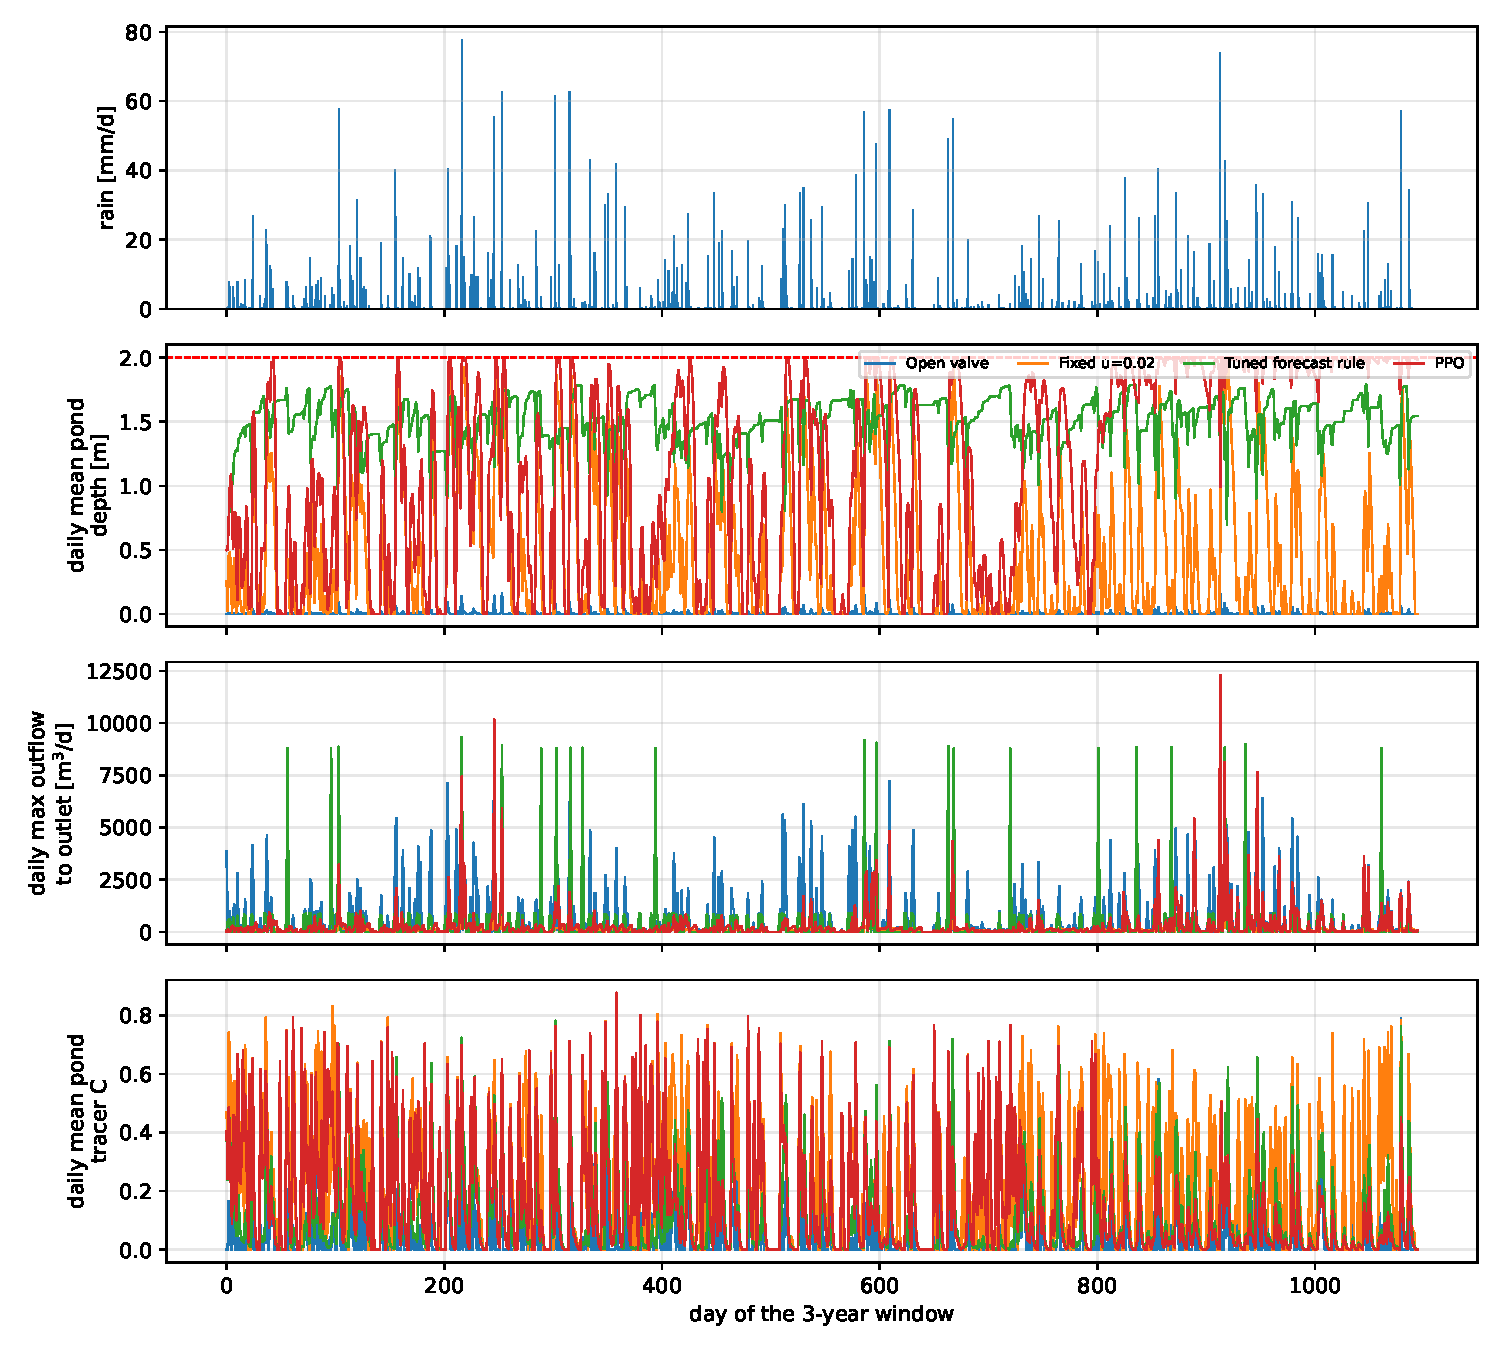
\includegraphics[width=0.92\textwidth]{figures/pond_trajectory_window0.pdf}
\caption{Test window 2020--2022, daily values. From top: daily rain; daily
mean pond depth (dashed: overflow crest); daily maximum flow to the outlet;
daily mean pond tracer concentration (lower means older water).}
\label{fig:pond_traj_w0}
\end{figure}

\begin{figure}[p]
\centering
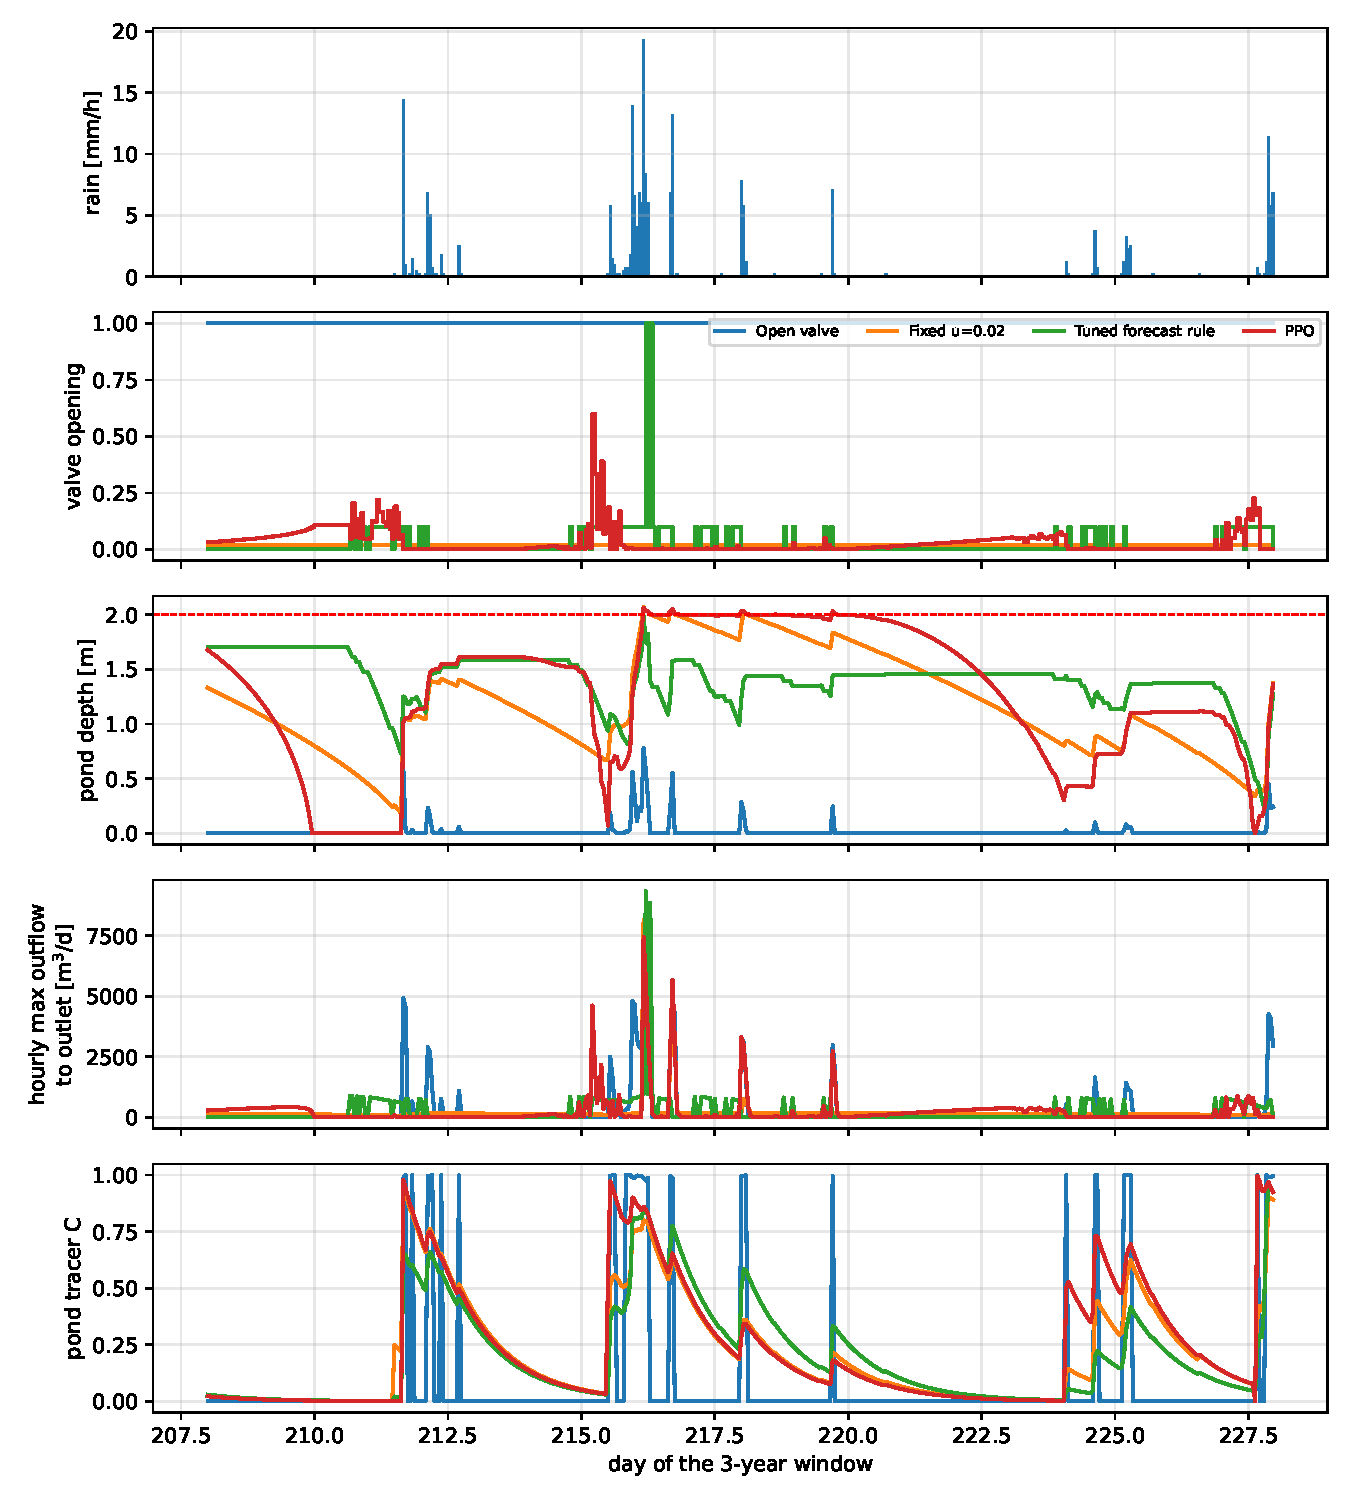
\includegraphics[width=0.92\textwidth]{figures/pond_trajectory_window0_zoom.pdf}
\caption{Test window 2020--2022, hourly detail of the 20 days around the
wettest day. From top: rain; valve opening; pond depth; hourly maximum flow
to the outlet; pond tracer concentration.}
\label{fig:pond_traj_w0_zoom}
\end{figure}

\begin{figure}[p]
\centering
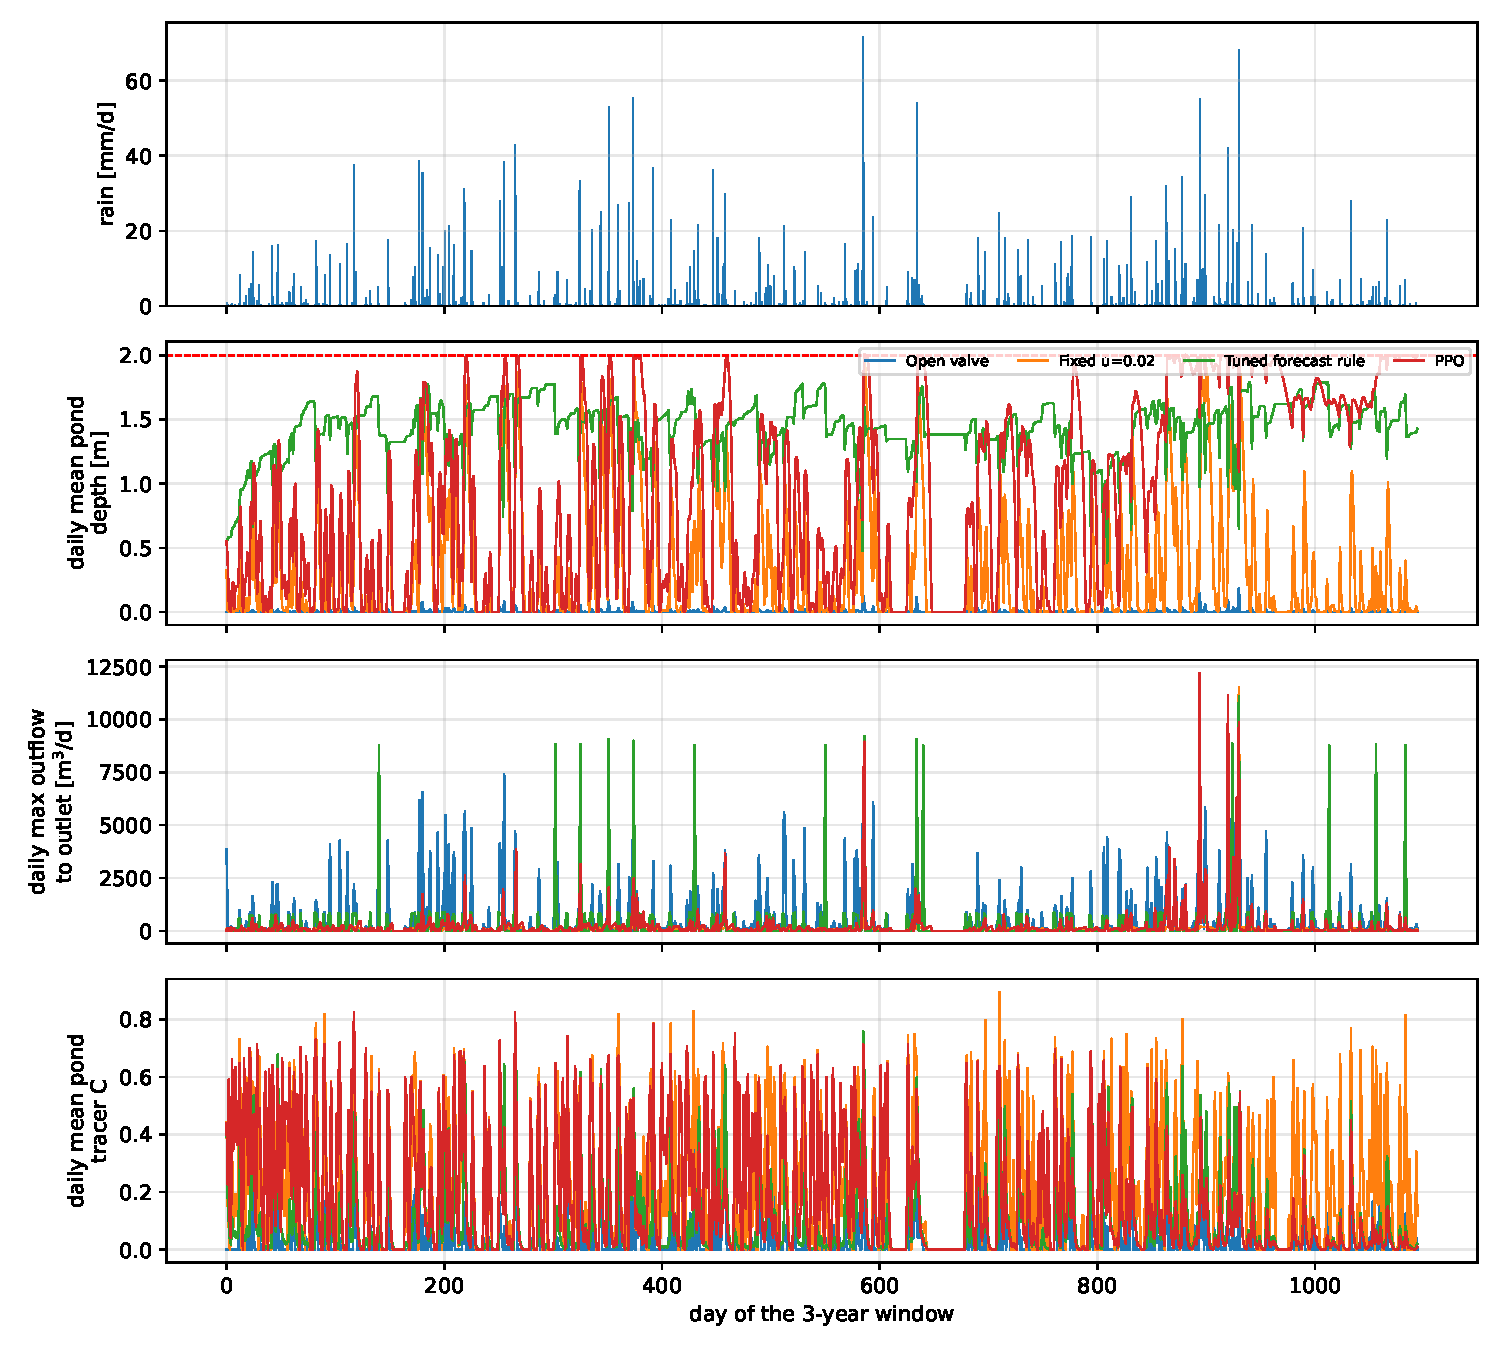
\includegraphics[width=0.92\textwidth]{figures/pond_trajectory_window1.pdf}
\caption{Test window 2023--2025, daily values (panels as in Figure~\ref{fig:pond_traj_w0}).}
\label{fig:pond_traj_w1}
\end{figure}

\begin{figure}[p]
\centering
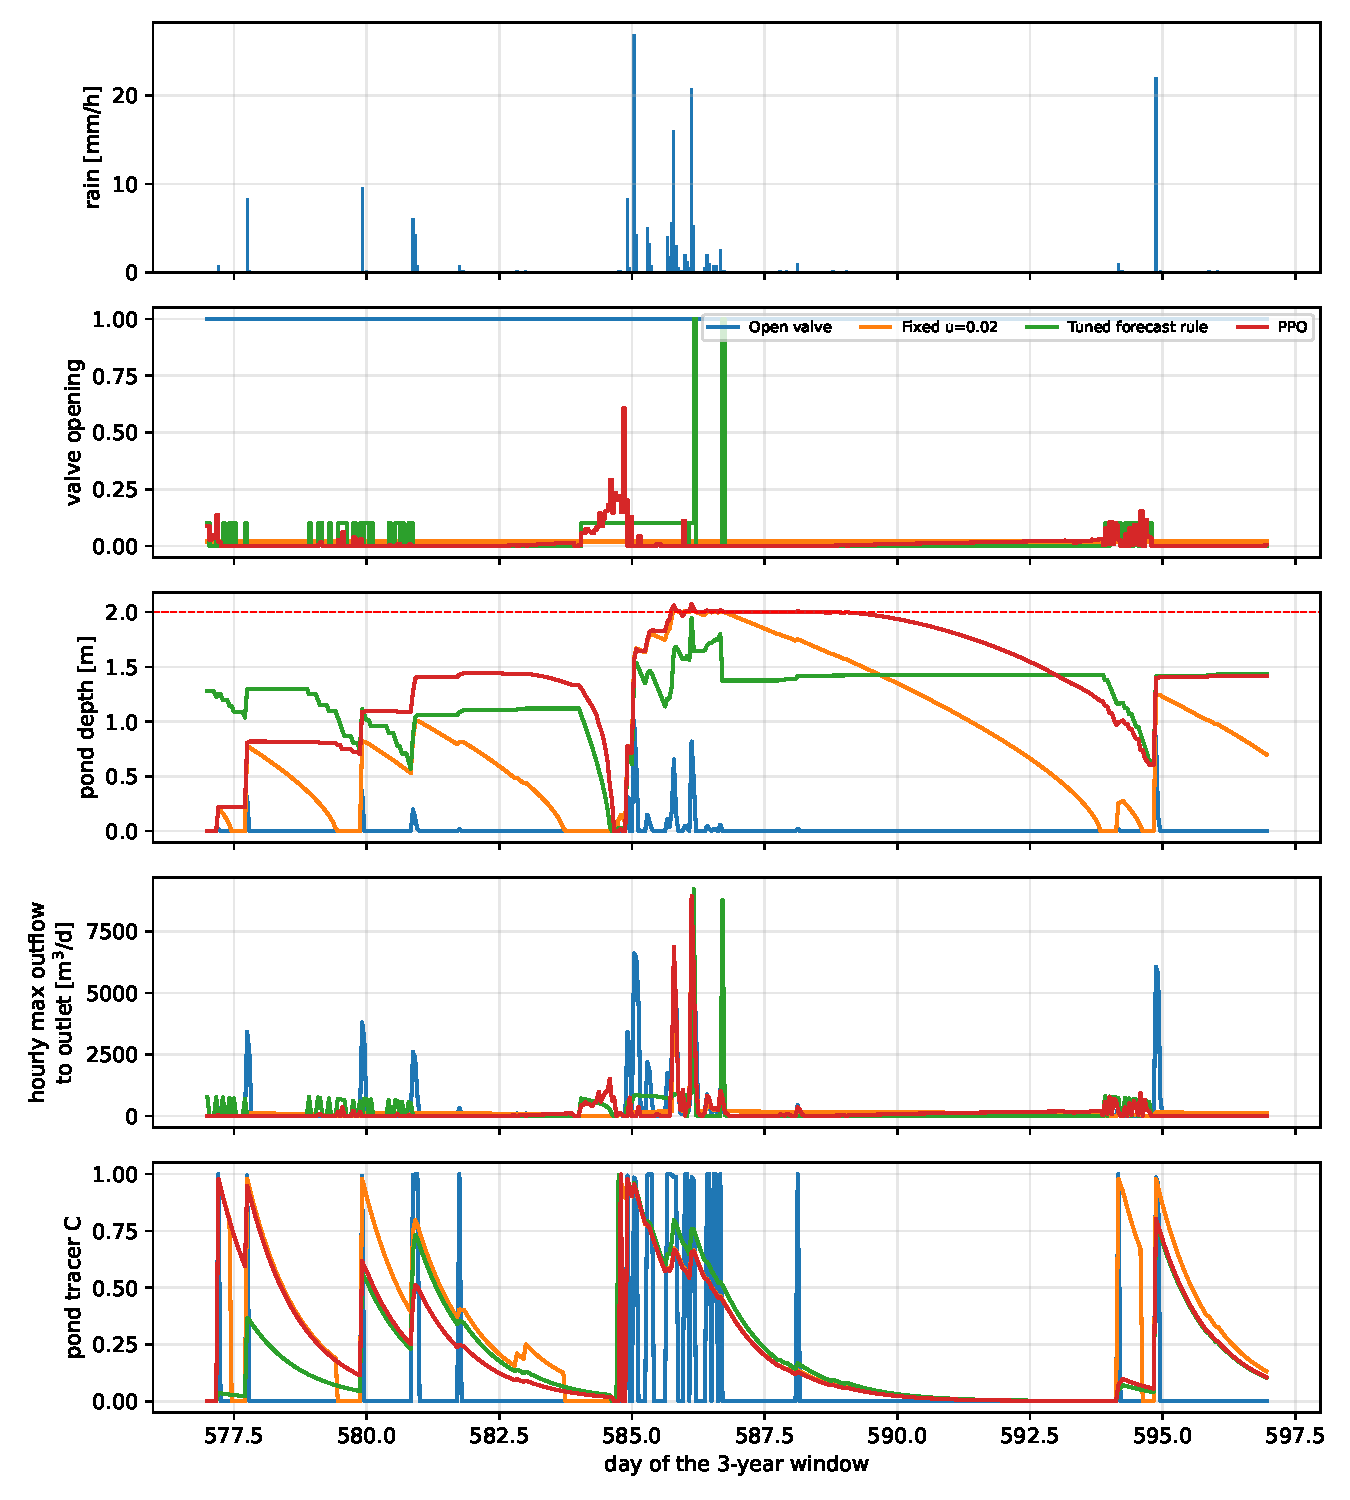
\includegraphics[width=0.92\textwidth]{figures/pond_trajectory_window1_zoom.pdf}
\caption{Test window 2023--2025, hourly detail around the wettest day.}
\label{fig:pond_traj_w1_zoom}
\end{figure}


%=====================================================================
\section{Limitations and next steps}
%=====================================================================
\begin{itemize}
\item \textbf{Make the problem harder than one rule can handle.} Candidates
are a cascade of reservoirs, a water-quality objective (OHQ's constituent
transport), hydropower with time-varying prices, or a longer,
skill-varying forecast. These are the settings where RL should pull ahead
of tuned rules.
\item \textbf{Simulator speed.} Replace \code{OHQBackend} with a
codegen-compiled kernel (Section~\ref{sec:performance}). Even within the
current bindings, a method to reset a block's state on a persistent
\code{System} and an in-memory output accessor would remove most of the
per-step overhead.
\item \textbf{OHQ fixes uncovered here.} (i) \emph{Done:} rebuilt
\code{libOHQLib} so the bindings use the end-of-step output stamping.
(ii) \emph{Open:} move the \code{"unit"} entry out of the \code{rule}
dictionary of \code{Reservoir\_link\_rule} in \code{main\_components.json}.
(iii) \emph{Done:} \code{SetSystemSettingsObjectProperties} returned
\code{false} whenever \code{settings.json} had not been loaded, even though
the value had been applied. It now returns \code{SetProperty}'s result
(branch \code{fix/set-system-value-return}), and the environment raises an
error if OHQ rejects a setting.
\item \textbf{RL details.} Training used a single seed and a fixed budget.
Multiple seeds, observation and reward normalization, and a tanh-squashed
policy would make the agent more robust. Daily-average flood accounting
also underweights sub-daily peaks; the reward could use the peak river flow
instead.
\end{itemize}

%=====================================================================
\section{How to reproduce}
%=====================================================================
\begin{lstlisting}[language=bash]
source ~/Projects/ohq_rl_env/bin/activate
cd ~/Projects/OpenHydroQual-RL
python diagnostics.py                       # verification + timing figures
python train_ppo.py --total-steps 409600 --num-envs 16 --out results/ppo_reservoir.pt
python evaluate.py --policy results/ppo_reservoir.pt --episodes 30
cd report && latexmk -pdf main.tex
\end{lstlisting}
The paths of the bindings and templates can be overridden with the
\code{OHQ\_PY\_PATH} and \code{OHQ\_RESOURCES} environment variables.

\section*{Appendix: RL glossary}
\addcontentsline{toc}{section}{Appendix: RL glossary}
\begin{description}\itemsep2pt\small
\item[Action ($a_t$)] What the agent decides at a step; here the release(s) for the day.
\item[Actor] The network that represents the policy, $o\mapsto\mu_\theta(o)$.
\item[Actor--critic] A method with both a policy network (actor) and a value network (critic). PPO is one.
\item[Advantage ($A$, $\hat A_t$)] How much better an action turned out than the policy's average in that situation; positive means ``do this more''.
\item[Agent] The decision maker; here the learned operating rule.
\item[Behavior cloning] Supervised training of the actor to imitate an existing policy (here the tuned rule) from its recorded observations and actions; used as a warm start for PPO.
\item[Baseline] (i) In this report: a comparison policy (demand only, rule curves). (ii) In RL theory: a function subtracted in the policy gradient to reduce noise; the critic plays this role.
\item[Bellman equation] The recursion ``value now = expected reward now + discounted value next'' (Eq.~\ref{eq:bellman}); the backbone of both SDP and RL.
\item[Bootstrapping] Building a value label partly from the critic's own prediction of the future, instead of waiting for all actual rewards.
\item[Clipping (PPO)] Limiting the change in action probabilities per update to $\pm\epsilon$ (20\%) so that learning is stable.
\item[Credit assignment] Working out which earlier actions caused a later reward or penalty.
\item[Critic] The value-function network $V_\phi(o)$ that predicts the return still to come.
\item[Discount factor ($\gamma$)] Weight $<1$ applied per step to future rewards; sets the effective planning horizon $\sim1/(1-\gamma)$ steps.
\item[Environment] Everything outside the agent: here the OHQ model plus the random storms and demand.
\item[Episode] One run from start to end; here one 90-day season.
\item[Epoch] One pass over the batch of collected data during an update.
\item[Exploration] Trying actions other than the current best guess, here through random noise around the mean action, to discover better behavior.
\item[GAE] Generalized advantage estimation: a weighted blend of multi-step TD errors (Eq.~\ref{eq:gae}).
\item[Generalization] Performing well on situations (seasons) not seen in training; tested on held-out seeds.
\item[Gymnasium] The standard Python interface for RL environments (\code{reset}, \code{step}).
\item[Hyperparameter] A setting of the learning algorithm itself (learning rate, $\gamma$, \dots), as opposed to the learned weights.
\item[Learning curve] Return versus amount of training experience.
\item[MDP] Markov decision process: states, actions, transition law, rewards; the mathematical model of a sequential decision problem.
\item[Minibatch] The subset of records used for one gradient step.
\item[Neural network] A flexible parametric function built from layers of simple nonlinear units; its weights are fitted by gradient descent.
\item[Observation ($o_t$)] The information the agent receives at a step; may be less than the full state.
\item[On-policy] Learning only from data collected by the current policy (PPO is on-policy, so it discards data after each update).
\item[Off-policy] Learning from data collected by older or other policies, typically stored in a replay memory (e.g.\ DQN, SAC); PPO is not off-policy.
\item[Policy ($\pi$)] The decision rule mapping observations to actions; stochastic during training, deterministic in evaluation.
\item[Policy gradient] The gradient of expected return with respect to the policy parameters (Eq.~\ref{eq:pg}); estimated from simulations without differentiating the simulator.
\item[PPO] Proximal Policy Optimization: the policy-gradient actor--critic algorithm used here.
\item[Replay memory] A store of past experience reused for many updates by off-policy methods; PPO has none and discards each batch after one update.
\item[Return] Sum of (possibly discounted) rewards over an episode; the quantity to maximize.
\item[Reward ($r_t$)] Scalar score of one step; its design defines the objective.
\item[Rollout] A stretch of simulated experience collected with the current policy.
\item[Seed] A number that fixes a random sequence; used to generate reproducible, distinct seasons.
\item[State ($s_t$)] Everything that determines the future evolution of the system.
\item[TD error ($\delta_t$)] One-step surprise: $r_t+\gamma V(o_{t+1})-V(o_t)$.
\item[Value function ($V^\pi$)] Expected return still to come from a state when following policy $\pi$.
\end{description}


\begin{thebibliography}{9}
\bibitem{schulman2017ppo} J.~Schulman, F.~Wolski, P.~Dhariwal, A.~Radford, O.~Klimov.
  Proximal Policy Optimization Algorithms. arXiv:1707.06347, 2017.
\bibitem{schulman2016gae} J.~Schulman, P.~Moritz, S.~Levine, M.~Jordan, P.~Abbeel.
  High-Dimensional Continuous Control Using Generalized Advantage Estimation. ICLR, 2016.
\end{thebibliography}

\end{document}
